%------------------------------------------------------------------------------
% Copyright (c) 1991-2014, Xavier Leroy and Didier Remy.  
%
% All rights reserved. Distributed under a creative commons
% attribution-non-commercial-share alike 2.0 France license.
% http://creativecommons.org/licenses/by-nc-sa/2.0/fr/
%
% Translation by Richard Paradies, reworked by Daniel C. Buenzli
%------------------------------------------------------------------------------

\chapter{\label{sec/files}Files}
\cutname{files.html}

The term \quotes{file} in Unix covers several types of objects:
%
\begin{itemize}
\item standard files: finite sets of bytes containing text or binary
  information, often referred to as \quotes{ordinary} files,
%
\item directories,
%
\item symbolic links,
%
\item special files (\emph{devices}), which primarily provide access
  to computer peripherals,
%
\item named pipes,
%
\item sockets named in the Unix domain.
\end{itemize}
% 
The file concept includes both the data contained in the file and
information about the file itself (also called meta-data) like its
type, its access rights, the latest access times, {\etc}

\section{The file system}

To a first approximation, the file system can be considered to be a tree. The root is
represented by \ml+'/'+. The branches are labeled by (file) names,
which are strings of any characters excluding \ml+'\000'+ and \ml+'/'+
(but it is good practice to also avoid non-printing characters and
spaces). The non-terminal nodes are \emph{directories}: these nodes
always contain two branches \ml+.+ and \ml+..+ which respectively
represent the directory itself and the directory's parent. The other
nodes are sometimes called \emph{files}, as opposed to directories,
but this is ambiguous, as we can also designate any node as a
\quotes{file}. To avoid all ambiguity we refer to them as
\emph{non-directory files}.

The nodes of the tree are addressed by paths. If the start of the path
is the root of the file hierarchy, the path is \emph{absolute}, whereas if the
start is a directory it is \emph{relative}. More precisely, a \emph{relative
  path} is a string of file names separated by the character
\ml+'/'+.  An \emph{absolute path} is a relative path preceded by the
the character \ml+'/'+ (note the double use of this character both as
a separator and as the name of the root node).

The \libmodule{Filename} module handles paths in a portable
manner. In particular, \libvalue{Filename}{concat} concatenates paths without
referring to the character \ml+'/'+, allowing the code to function equally
well on other operating systems (for example, the path separator character
under Windows is \ml+'\'+).  Similarly, the \ml+Filename+ module
provides the string values \libvalue{Filename}{current\_dir\_name} and
\libvalue{Filename}{parent\_dir\_name} to represent the branches
\ml+.+ and \ml+..+ The functions \libvalue{Filename}{basename} and
\libvalue{Filename}{dirname} return the prefix \ml+d+ and the suffix
\ml+b+ from a path \ml+p+ such that the paths \ml+p+ and
\ml+d/b+ refer to the same file, where \ml+d+ is the directory in
which the file is found and \ml+b+ is the name of the file. The
functions defined in \ml+Filename+ operate only on paths,
independently of their actual existence within the file hierarchy.

In fact, strictly speaking, the file hierarchy is not a tree. First
the directories \ml+.+ and \ml+..+ allow a directory to refer to
itself and to move up in the hierarchy to define paths leading from a
directory to itself. Moreover, non-directory files can have many
parents (we say that they have many \emph{hard links}). Finally,
there are also \emph{symbolic links} which can be seen as
non-directory files containing a path. Conceptually, this path can be
obtained by reading the contents of the symbolic link like an ordinary
file. Whenever a symbolic link occurs in the middle of a path we have
to follow its path transparently. If \ml+s+ is a symbolic link whose
value is the path \ml+l+, then the path \ml+p/s/q+ represents the file
\ml+l/q+ if \ml+l+ is an absolute path or the file \ml+p/l/q+ if
\ml+l+ is a relative path.

Figure~\ref{fig/hierarchy} gives an example of a file hierarchy.  The
symbolic link \ml+11+ corresponding to the path \ml+/tmp/bar+ whose
path value is the relative path \ml+../gnu+, does not refer to any
existing file in the hierarchy (at the moment).

\begin{myfigure}
\begin{myimage}[width="100\%"]
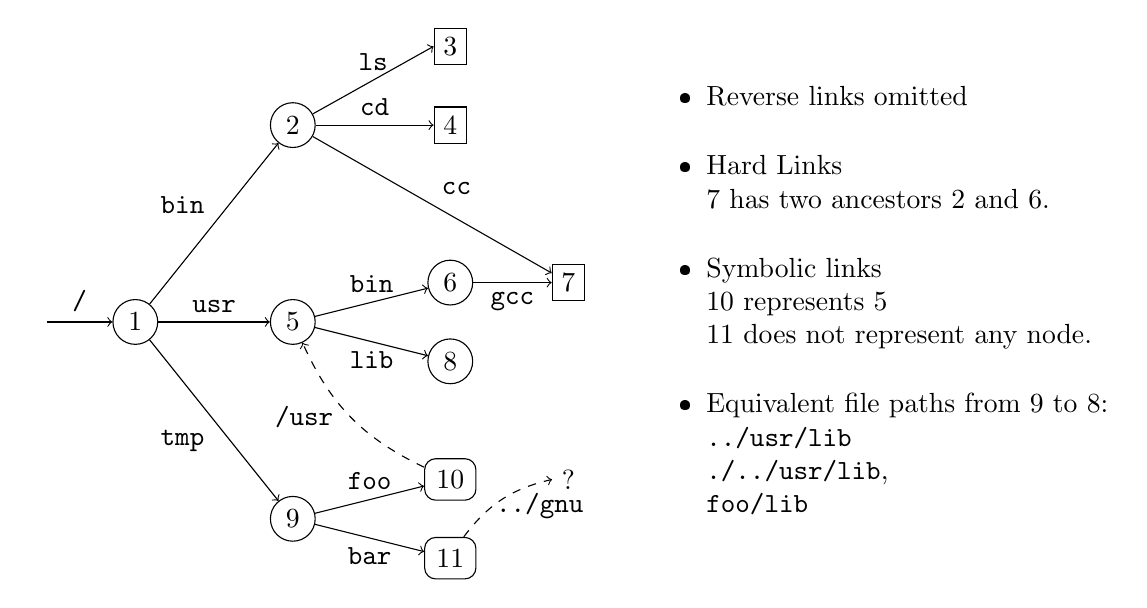
\begin{tikzpicture}
[dir/.style={draw, circle, inner sep=1mm},
 slink/.style={draw,rectangle,inner sep=1.5mm, rounded corners},
 file/.style={draw,rectangle},
 tpath/.style={font={\ttfamily},midway}]
\node (start) at (-1.25,0) {};
\node (n1) at (0,0) [dir] {1};

\node (n2) at (2,2.5) [dir] {2};
\node (n5) at (2,0) [dir] {5};
\node (n9) at (2,-2.5) [dir] {9};

\node (n3) at (4,3.5) [file] {3};
\node (n4) at (4,2.5) [file] {4};
\node (n6) at (4,0.5) [dir] {6};
\node (n8) at (4,-0.5) [dir] {8};
\node (n10) at (4, -2) [slink] {10};
\node (n11) at (4, -3) [slink] {11};

\node (n7) at (5.5, 0.5) [file] {7};
\node (nqmark) at (5.5, -2) {?};

\draw[->] (start) to node [tpath,above] {/} (n1);

\draw[->] (n1) to node [tpath,above left] {bin} (n2);
\draw[->] (n1) to node [tpath,above] {usr} (n5);
\draw[->] (n1) to node [tpath,below left] {tmp} (n9);

\draw[->] (n2) to node [tpath,above] {ls} (n3.west);
\draw[->] (n2) to node [tpath,above] {cd} (n4);
\draw[->] (n2) to node [tpath,above right] {cc} (n7);

\draw[->] (n5) to node [tpath,above] {bin} (n6);
\draw[->] (n5) to node [tpath,below] {lib} (n8);

\draw[->] (n9) to node [tpath,above] {foo} (n10);
\draw[->] (n9) to node [tpath,below] {bar} (n11);

\draw[->] (n6) to node [tpath,below] {gcc} (n7);

\draw[->,dashed] (n10) to [bend left=20] node [tpath,left=1mm] {/usr} (n5);
\draw[->,dashed] (n11) to [bend left=20] node [tpath,below right=-2mm] {../gnu} (nqmark.west);
\node[right=0.75cm, text width=6cm] at (n7)
{
  \begin{itemize}
    \item Reverse links omitted \vspace{5pt}
    \item Hard Links \\ 
      7 has two ancestors 2 and 6.\vspace{5pt}
    \item Symbolic links \\ 
      10 represents 5 \\ 
      11 does not represent any node. \vspace{5pt}
    \item Equivalent file paths from  9 to 8: \\
      \texttt{../usr/lib} \\
      \texttt{./../usr/lib}, {\etc} \\
      \texttt{foo/lib}
  \end{itemize}
};
\end{tikzpicture}
\end{myimage}
\caption{An example of a file hierarchy}
\label{fig/hierarchy}
\end{myfigure}

In general, a recursive traversal of the hierarchy will terminate
if the following rules are respected:
%
\begin{itemize}
\item the directories \ml+.+ and \ml+..+ are ignored.
\item symbolic links are not followed. 
\end{itemize}
% 
But if symbolic links are followed we are traversing a graph and
we need to keep track of the nodes we have already visited to avoid loops.

Each process has a current working directory. It is returned by the
function \indexlibvalue{Unix}{getcwd} and can be changed with
\indexlibvalue{Unix}{chdir}.  It is also possible to constrict the
view of the file hierarchy by calling 
\indexlibvalue{Unix}{chroot} \ml+p+. This makes the node \ml+p+, which 
should be a directory, the root of the restricted view of the
hierarchy. Absolute file paths are then
interpreted according to this new root \ml+p+ (and of course \ml+..+ at the
new root is \ml+p+ itself).

\section{File names and file descriptors}

There are two ways to access a file.  The first is by its \emph{file
  name} (or \emph{path name}) in the file system hierarchy.  Due to
hard links, a file can have many different names.  Names are values of
type \ml+string+. For example the system calls \syscall{unlink},
\syscall{link}, \syscall{symlink} and \syscall{rename} all operate at
the file name level.
%
\begin{listingcodefile}{tmpunix.mli}
val $\libvalue{Unix}{unlink}$ : string -> unit
val $\libvalue{Unix}{link}$ : string -> string -> unit
val $\libvalue{Unix}{symlink}$ : string -> string -> unit
val $\libvalue{Unix}{rename}$ : string -> string -> unit
\end{listingcodefile}
% 
Their effect is as follows:
\begin{itemize}
\item \ml+unlink f+ erases the file \ml+f+ like the Unix command
\ml+rm -f f+.
%
\item \ml+link f1 f2+ creates a hard link named \ml+f2+ to
the file \ml+f1+ like the command \ml+ln f1 f2+.
%
\item \ml+symlink f1 f2+ creates a symbolic link named \ml+f2+ to the file 
\ml+f1+ like the command \ml+ln -s f1 f2+. 
%
\item \ml+rename f1 f2+ renames the file \ml+f1+ to \ml+f2+ 
like the command \ml+mv f1 f2+.
\end{itemize}

The second way of accessing a file is by a file descriptor. A
descriptor represents a pointer to a file along with other information
like the current read/write position in the file, the access rights of
the file (is it possible to read? write?) and flags which control the
behavior of reads and writes (blocking or non-blocking, overwrite,
append, \etc). File descriptors are values of the abstract type
\libtype{Unix}{file\_descr}.

Access to a file via its descriptor is independent from the
access via its name. In particular whenever we get a file descriptor,
the file can be destroyed or renamed but the descriptor still points
on the original file.

When a program is executed, three descriptors are allocated and 
tied to the variables \ml+stdin+, \ml+stdout+ and \ml+stderr+ of the
\ml+Unix+ module:
\begin{codefile}{tmpunix.mli}
type file_descr
\end{codefile}
\begin{listingcodefile}{tmpunix.mli}
val $\indexlibvalue{Unix}{stdin}$ : file_descr
val $\indexlibvalue{Unix}{stdout}$ : file_descr
val $\indexlibvalue{Unix}{stderr}$ : file_descr
\end{listingcodefile}
They correspond, respectively, to the standard input, standard output
and standard error of the process.

When a program is executed on the command line without any
redirections, the three descriptors refer to the terminal.  But if,
for example, the input has been redirected using the shell expression
\ml+cmd < f+, then the descriptor \ml+stdin+ refers to the file named \ml+f+
during the execution of the command \ml+cmd+. Similarly, \ml +cmd > f+
and \ml+cmd 2> f+ respectively bind the descriptors \ml+stdout+ and
\ml+stderr+ to the file named \ml+f+ during the execution of the
command.


\section{Meta-attributes, types and permissions}

The system calls \syscall{stat}, \syscall{lstat} and \syscall{fstat}
return the meta-attributes of a file; that is, information about
the node itself rather than its content. Among other things, this
information contains the identity of the file, the type of file, the
access rights, the time and date of last access and other information.
%
\begin{codefile}{tmpunix.mli}
type stats
\end{codefile}
%
\begin{listingcodefile}{tmpunix.mli}
val $\libvalue{Unix}{stat}$  : string -> stats
val $\libvalue{Unix}{lstat}$ : string -> stats
val $\libvalue{Unix}{fstat}$ : file_descr -> stats
\end{listingcodefile}
% 
The system calls \ml+stat+ and \ml+lstat+ take a file name as an
argument while \ml+fstat+ takes a previously opened descriptor and
returns information about the file it points to.  \ml+stat+ and
\ml+lstat+ differ on symbolic links : \ml+lstat+ returns information
about the symbolic link itself, while \ml+stat+ returns information
about the file that the link points to. The result of these three
calls is a record of type \libtype{Unix}{stats} whose fields are
described in table~\ref{fig/stats}.
%
\begin{mytable}
\begin{tabular}{lp{9cm}}
Field name & Description \\
%
\hline
\ml+st_dev : int+ 
& The id of the device on which the file is stored. \\
%
\ml+st_ino : int+ 
& The id of the file (inode number) in its partition. 
The pair \ml+(st_dev, st_ino)+ uniquely identifies the file
within the file system. \\
%
\ml+st_kind : file_kind+ & 
The file type. The type \libtype{Unix}{file\_kind} is an enumerated type
whose constructors are:  
\begin{mltypecases}
\begin{tabular}{@{}ll}
\ml+S_REG+ & Regular file \\
\ml+S_DIR+ & Directory \\
\ml+S_CHR+ & Character device  \\
\ml+S_BLK+ & Block device  \\
\ml+S_LNK+ & Symbolic link \\
\ml+S_FIFO+ & Named pipe \\
\ml+S_SOCK+ & Socket 
\end{tabular}
\end{mltypecases}
\\
%
\ml+st_perm : int+ & Access rights for the file \\
%
\ml+st_nlink : int+ 
& For a directory: the number of entries in the directory. For others:
the number of hard links to this file. \\
%
\ml+st_uid : int+ & The id of the file's user owner. \\
%
\ml+st_gid : int+ & The id of the file's group owner. \\
%
\ml+st_rdev : int+ 
& The id of the associated peripheral (for special files). \\
%
\ml+st_size : int+ & The file size, in bytes. \\
%
\ml+st_atime : int+ & Last file content access date (in seconds from
January 1st 1970, midnight, \textsc{gmt}). \\
%
\ml+st_mtime : int+ & Last file content modification date (idem).\\
%
\ml+st_ctime : int+ & Last file state modification date: either a
write to the file or a change in access rights, user or group owner,
or number of links.
\smallskip\\
\hline
\end{tabular}
\caption{Fields of the \ml+stats+ structure}
\label{fig/stats}
\end{mytable}

\subsection*{Identification}

A file is uniquely identified by the pair made of its device number
(typically the disk partition where it is located) \ml+st_dev+ and its
inode number \ml+st_ino+.

\subsection*{Owners}

A file has one user owner \ml+st_uid+ and one group owner
\ml+st_gid+.  All the users and groups 
on the machine are usually described in the  
 \ml+/etc/passwd+ and \ml+/etc/groups+ files. We can look up them by
name in a portable manner with the functions \syscall{getpwnam} and 
\syscall{getgrnam} or by id with 
\syscall{getpwuid} and \syscall{getgrgid}.
%
\begin{codefile}{tmpunix.mli}
type passwd_entry = Unix.passwd_entry
type group_entry = Unix.group_entry
\end{codefile}
%
\begin{listingcodefile}{tmpunix.mli}
val $\libvalue{Unix}{getpwnam}$ : string -> passwd_entry
val $\libvalue{Unix}{getgrnam}$ : string -> group_entry
val $\libvalue{Unix}{getpwuid}$ : int -> passwd_entry
val $\libvalue{Unix}{getgrgid}$ : int -> group_entry
\end{listingcodefile}

The name of the user of a running process and all the groups
to which it belongs can be retrieved with the commands
\syscall{getlogin} and \syscall{getgroups}.
%
\begin{listingcodefile}{tmpunix.mli}
val $\libvalue{Unix}{getlogin}$ : unit -> string
val $\libvalue{Unix}{getgroups}$ : unit -> int array
\end{listingcodefile}

The call \syscall{chown} changes the owner (second argument) and the
group (third argument) of a file (first argument). If we have a file
descriptor, \syscall{fchown} can be used instead. Only the super user
can change this information arbitrarily.
%
\begin{listingcodefile}{tmpunix.mli}
val $\libvalue{Unix}{chown}$ : string -> int -> int -> unit
val $\libvalue{Unix}{fchown}$ : file_descr -> int -> int -> unit
\end{listingcodefile}

%% Le changement de groupe peut se faire sans privilège lorsque le
%% programme à un \ml+uid+ (effectif) égal à celui du fichier et un
%% \ml+gid+ (effectif) égal au group désiré ou à un de ses groupes
%% supplémentaire

\subsection*{Access rights}

Access rights are encoded as bits in an integer, and the type
\libtype{Unix}{file\_perm} is just an abbreviation for the type
\ml+int+. They specify special bits and read, write and
execution rights for the user owner, the group owner and the other
users as vector of bits:
%
\ifhtmlelse{%
\begin{center}
\begin{tabular}{ccc|ccc|ccc|ccc}
\multicolumn{3}{c}{\texttt{S}pecial}
&\multicolumn{3}{c}{\texttt{U}ser}
&\multicolumn{3}{c}{\texttt{G}roup}
&\multicolumn{3}{c}{\texttt{O}ther} \\
\hline
--&--&--&--&--&--&--&--&--&--&--&--\\
\hline
\multicolumn{12}{c}{\ml+OoSUGO+}
\end{tabular}
\end{center}
}
{%
\begin{displaymath}
\underbrace
{\overbrace{---}^{\texttt Special}
 \overbrace{---}^{\texttt User}
 \overbrace{---}^{\texttt Group}
 \overbrace{---}^{\texttt Other}}_{\texttt{0oSUGO}}
\end{displaymath}
}
% 
where in each of the user, group and other fields, the order of bits
indicates read (\ml+r+), write (\ml+w+) and execute (\ml+x+) rights.
The permissions on a file are the union of all these individual
rights, as shown in table~\ref{tab/permbits}.

\begin{mytable}
\begin{tabular}{lcl}
Bit (octal) & Notation \ml+ls -l+ & Access right \\
\hline
\ml+0o100+ & \ml+--x------+ & executable by the user owner \\
\ml+0o200+ & \ml+-w-------+ & writable by the user owner \\
\ml+0o400+ & \ml+r--------+ & readable by the user owner \\
\hline
\ml+0o10+  & \ml+-----x---+ &
        executable by members of the group owner \\
\ml+0o20+  & \ml+----w----+ &
        writable by members of the group owner \\
\ml+0o40+  & \ml+---r----+ &
        readable by members of the group owner \\
\hline
\ml+0o1+   & \ml+--------x+ & executable by other users\\
\ml+0o2+   & \ml+-------w-+ & writable by other users \\
\ml+0o4+   & \ml+------r--+ & readable by other users \\
\hline
\ml+0o1000+ & \ml+--------t+ & the bit \ml+t+ on the group (sticky bit)\\
\ml+0o2000+ & \ml+-----s---+ & the bit \ml+s+ on the group (\ml+set-gid+)\\
\ml+0o4000+ & \ml+--s------+ & the bit \ml+s+ on the user (\ml+set-uid+)\\
\hline
\end{tabular}
\caption{Permission bits}\label{tab/permbits}
\end{mytable}

For files, the meaning of read, write and execute permissions is
obvious. For a directory, the execute permission means the right to
enter it (to \ml+chdir+ to it) and read permission the right to list
its contents. Read permission on a directory is however not needed to
read its files or sub-directories (but we then need to know their
names).

The special bits do not have meaning unless the \ml+x+ bit is set (if
present without \ml+x+ set, they do not give additional rights).  This
is why their representation is superimposed on the bit \ml+x+ and
the letters \ml+S+ and \ml+T+ are used instead of \ml+s+ and \ml+t+
whenever \ml+x+ is not set. The bit \ml+t+ allows sub-directories to
inherit the permissions of the parent directory. On a directory, 
the bit \ml+s+ allows the use of the directory's \ml+uid+ or \ml+gid+ rather
than the user's to create directories. For an executable file, 
the bit \ml+s+ allows the changing at execution time of the user's
effective identity or group with the system calls \syscall{setuid} 
and \syscall{setgid}.
%
\begin{listingcodefile}{tmpunix.mli}
val $\libvalue{Unix}{setuid}$ : int -> unit
val $\libvalue{Unix}{setgid}$ : int -> unit
\end{listingcodefile}
%
The process also preserves its original identities unless 
it has super user privileges, in which case \ml+setuid+ and
\ml+setgid+ change both its effective and original user and group
identities. The original identity is preserved to allow 
the process to subsequently recover it as its effective identity
without needing further privileges. The system calls \syscall{getuid} and 
\syscall{getgid} return the original identities and 
\syscall{geteuid} and \syscall{getegid} return the effective identities.
%
\begin{listingcodefile}{tmpunix.mli}
val $\libvalue{Unix}{getuid}$ : unit -> int
val $\libvalue{Unix}{geteuid}$ : unit -> int
val $\libvalue{Unix}{getgid}$ : unit -> int
val $\libvalue{Unix}{getegid}$ : unit -> int
\end{listingcodefile}

A process also has a file creation mask encoded the same way file
permissions are. As its name suggests, the mask specifies prohibitions
(rights to remove): during file creation a bit set to 1 in the
mask is set to 0 in the permissions of the created file.  The mask
can be consulted and changed with the system call \syscall{umask}:
%
\begin{listingcodefile}{tmpunix.mli}
val $\libvalue{Unix}{umask}$ : int -> int
\end{listingcodefile}
% 
Like many system calls that modify system variables, the modifying
function returns the old value of the variable. Thus, to just look up
the value we need to call the function twice. Once with an arbitrary
value to get the mask and a second time to put it back. For example:
%
\begin{codefile}{tmpfich.ml}
open Unix;;
let _ = 
\end{codefile}
%
\begin{listingcodefile}{tmpfich.ml}
let m = umask 0 in ignore (umask m); m
\end{listingcodefile}

File access permissions can be modified with the system calls
\syscall{chmod} and \syscall{fchmod}:
%
\begin{codefile}{tmpunix.mli}
type file_perm
\end{codefile}
%
\begin{listingcodefile}{tmpunix.mli}
val $\libvalue{Unix}{chmod}$ : string -> file_perm -> unit
val $\libvalue{Unix}{fchmod}$ : file_descr -> file_perm -> unit
\end{listingcodefile}
and they can be tested \quotes{dynamically} with the system 
call \syscall{access}:
%
\begin{listingcodefile}{tmpunix.mli}
type $\libtype{Unix}{access\_permission}$ = R_OK | W_OK | X_OK | F_OK
val $\libvalue{Unix}{access}$ : string -> access_permission list -> unit 
\end{listingcodefile}
%
where requested access rights to the file are specified by a list of
values of type \libtype{Unix}{access\_permission} whose meaning is 
obvious except for \ml+F_OK+ which just checks for the file's
existence (without checking for the other rights). The function
raises an error if the access rights are not granted.

Note that the information inferred by \ml+access+ may be more
restrictive than the information returned by \ml+lstat+ because a file
system may be mounted with restricted rights~---~for example in
read-only mode. In that case \ml+access+ will deny a write permission
on a file whose meta-attributes would allow it. This is why we
distinguish between \quotes{dynamic} (what a process can actually do)
and \quotes{static} (what the file system specifies) information.

\section{Operations on directories}

Only the kernel can write in directories (when files are
created). Thus opening a directory in write mode is prohibited. In
certain versions of Unix a directory may be opened in read only mode
and read with \indexvalue{read}, but other versions prohibit
it. However, even if this is possible, it is preferable not to do so
because the format of directory entries vary between Unix versions and
is often complex. The following functions allow reading a directory
sequentially in a portable manner:
%
\begin{codefile}{tmpunix.mli}
type dir_handle = Unix.dir_handle
\end{codefile}
%
\begin{listingcodefile}{tmpunix.mli}
val $\libvalue{Unix}{opendir}$   : string -> dir_handle
val $\libvalue{Unix}{readdir}$   : dir_handle -> string
val $\libvalue{Unix}{rewinddir}$ : dir_handle -> unit
val $\libvalue{Unix}{closedir}$  : dir_handle -> unit
\end{listingcodefile}
% 
The system call \syscall{opendir} returns a directory descriptor for a
directory. \syscall{readdir} reads the next entry of a descriptor, and
returns a file name relative to the directory or raises the exception
\ml+End_of_file+ if the end of the directory is
reached. \syscall{rewinddir} repositions the descriptor at the
beginning of the directory and \syscall{closedir} closes the directory
descriptor.

\begin{example}
The following library function, in \ml+Misc+, iterates a
function \ml+f+ over the entries of the directory \ml+dirname+.
%
\begin{codefile}{misc.mli}
(*** Directory iterator *)
val iter_dir : (string -> 'a) -> string -> unit
(** [iter_dir f d] opens path [d] as a directory and iterates the 
function [f] over all its entries *)
\end{codefile}
%
\begin{codefile}{misc.ml}
open Sys;;
open Unix;;
\end{codefile}
%
\begin{listingcodefile}{misc.ml}
let iter_dir f dirname =
  let d = opendir dirname in
  try while true do f (readdir d) done
  with End_of_file -> closedir d
\end{listingcodefile}
\end{example}

To create a directory or remove an empty directory, we have
\syscall{mkdir} and \syscall{rmdir}:
%
\begin{listingcodefile}{tmpunix.mli}
val $\libvalue{Unix}{mkdir}$ : string -> file_perm -> unit
val $\libvalue{Unix}{rmdir}$ : string -> unit
\end{listingcodefile}
% 
The second argument of \ml+mkdir+ determines the access rights of the
new directory.  Note that we can only remove a directory that is
already empty. To remove a directory and its contents, it is thus
necessary to first recursively empty the contents of the directory and
then remove the directory.

\section{\label{ex/find}Complete example: search in a file hierarchy}

The Unix command \ml+find+ lists the files of a hierarchy matching
certain criteria (file name, type and permissions \etc). In this
section we develop a library function \ml+Findlib.find+ which
implements these searches and a command \ml+find+ that provides a version
of the Unix command \ml+find+ that supports the options \ml+-follow+
and \ml+-maxdepth+.

We specify the following interface for \ml+Findlib.find+:
%
\begin{listingcodefile}{findlib.mli}
val find : 
  (Unix.error * string * string -> unit) -> 
  (string -> Unix.stats -> bool) -> bool -> int -> string list -> 
  unit
\end{listingcodefile}
%
The function call
\begin{lstlisting}
find handler action follow depth roots
\end{lstlisting}
traverses the file hierarchy starting from the roots specified in the
list \ml+roots+ (absolute or relative to the current directory of the
process when the call is made) up to a maximum depth \ml+depth+ and following
symbolic links if the flag \ml+follow+ is set.  The paths found under
the root \ml+r+ include \ml+r+ as a prefix.  Each found path \ml+p+ is
given to the function \ml+action+ along with the data returned by
\ml+Unix.lstat p+ (or \ml+Unix.stat p+ if \ml+follow+ is \ml+true+).
The function \ml+action+ returns a boolean indicating, for
directories, whether the search should continue for its contents (\ml+true+)
or not (\ml+false+).

The \ml+handler+ function reports traversal errors of type
\ml+Unix_error+. Whenever an error occurs the arguments of the
exception are given to the handler function and the traversal
continues. However when an exception is raised by the functions
\ml+action+ or \ml+handler+ themselves, we immediately stop the
traversal and let it propagate to the caller. To propagate an
\ml+Unix_error+ exception without catching it like a traversal error,
we wrap these exceptions in the \ml+Hidden+ exception (see
\ml+hide_exn+ and \ml+reveal_exn+).
%
%%% commented in the french version
%% De plus on arrête la visite récursive d'un répertoire que l'on est en train
%% de visiter (ce qui ne peut arriver que lorsqu'on suit les liens symboliques)
\begin{listingcodefile}[style=numbers]{findlib.ml}
open Unix;;

exception Hidden of exn
let hide_exn f x = try f x with exn -> raise (Hidden exn);;
let reveal_exn f x = try f x with Hidden exn -> raise exn;;

let find on_error on_path follow depth roots =
  let rec find_rec depth visiting filename =
    try
      let infos = (if follow then stat else lstat) filename in
      let continue = hide_exn (on_path filename) infos in
      let id = infos.st_dev, infos.st_ino in $\label{prog:did}$
      if infos.st_kind = S_DIR && depth > 0 && continue &&
        (not follow || not (List.mem id visiting))
      then
        let process_child child = 
          if (child <> Filename.current_dir_name &&
              child <> Filename.parent_dir_name) then 
            let child_name = Filename.concat filename child in
            let visiting = 
              if follow then id :: visiting else visiting in $\label{prog:follow}$
            find_rec (depth-1) visiting child_name in
        Misc.iter_dir process_child filename 
    with Unix_error (e, b, c) -> hide_exn on_error (e, b, c) in
  reveal_exn (List.iter (find_rec depth [])) roots;;
\end{listingcodefile}

A directory is identified by the \ml+id+ pair (line~\ref{prog:did})
made of its device and inode number.  The list \ml+visiting+ keeps
track of the directories that have already been visited. In fact
this information is only needed if symbolic links are followed
(line~\ref{prog:follow}).

It is now easy to program the \ml+find+ command. The essential part of
the code parses the command line arguments with the \libmodule{Arg}
module.
\begin{listingcodefile}{find.ml}
let find () =
  let follow = ref false in
  let maxdepth = ref max_int in
  let roots = ref [] in
  let usage_string  =
    ("Usage: " ^ Sys.argv.(0) ^ " [files...] [options...]") in
  let opt_list =  [ 
    "-maxdepth", Arg.Int ((:=) maxdepth), "max depth search";
    "-follow", Arg.Set follow, "follow symbolic links";
  ] in
  Arg.parse opt_list (fun f -> roots := f :: !roots) usage_string;
  let action p infos = print_endline p; true in
  let errors = ref false in
  let on_error (e, b, c) =
    errors := true; prerr_endline (c ^ ": " ^ Unix.error_message e) in
  Findlib.find on_error action !follow !maxdepth 
    (if !roots = [] then [ Filename.current_dir_name ] 
     else List.rev !roots);
  if !errors then exit 1;; 

Unix.handle_unix_error find ();;
\end{listingcodefile}
%
\begin{codefile}{find.test}
cd ../../lib/arch
./find.byte -follow -maxdepth 10 A B > find.out
find A B -follow -maxdepth 10 | diff - find.out
rm find.out
\end{codefile}
Although our \ml+find+ command is quite limited, the library
function \ml+FindLib.find+ is far more general, as the following
exercise shows.
\begin{exercise}
Use the function \ml+FindLib.find+ to write a command
\ml+find_but_CVS+ equivalent to the Unix command:
\begin{lstlisting}
find . -type d -name CVS -prune -o -print
\end{lstlisting}
which, starting from the current directory, recursively prints
files without printing or entering directories whose name is \ml+CVS+.
\end{exercise}
\begin{answer}
\begin{codefile}{find_but_CVS.ml}
open Unix;;
open Misc;;
\end{codefile}
%
\begin{listingcodefile}{find_but_CVS.ml}
let main () = 
  let action p infos = 
    let b = not (infos.st_kind = S_DIR || Filename.basename p = "CVS") in
    if b then print_endline p; b in
  let errors = ref false in
  let error (e,c,b) = 
    errors:= true; prerr_endline (b ^ ": " ^ error_message e) in
  Findlib.find error action false max_int [ "." ];;
handle_unix_error main ()
\end{listingcodefile}
\end{answer}

\begin{exercise}
The function \ml+getcwd+ is not a system call but is defined in the
\ml+Unix+ module.  Give a \quotes{primitive} implementation of
\ml+getcwd+. First describe the principle of your algorithm with words
and then implement it (you should avoid repeating the same system
call).
\end{exercise}
\begin{answer}
Here are some hints. We move up from the current position towards the
root and construct backwards the path we are looking for. The root can
be detected as the only directory node whose parent is equal to itself
(relative to the root \ml+.+ and \ml+..+ are equal). To find the name
of a directory \ml+r+ we need to list the contents of its parent
directory and detect the file that corresponds to \ml+r+.
\end{answer}

\section{Opening a file}

The \ml+openfile+ function allows us to obtain a descriptor for
a file of a given name (the corresponding system call
is \syscall{open}, however \ml+open+ is a keyword in {\ocaml}).
%
\begin{codefile}{tmpunix.mli}
type open_flag = Unix.open_flag;;
\end{codefile}
%
\begin{listingcodefile}{tmpunix.mli}
val $\libvalue{Unix}{openfile}$ : 
 string -> open_flag list -> file_perm -> file_descr
\end{listingcodefile}
% 
The first argument is the name of the file to open. The second
argument, a list of flags from the enumerated type
\libtype{Unix}{open\_flag}, describes the mode in which the file should
be opened and what to do if it does not exist. The third argument of
type \libtype{Unix}{file\_perm} defines the file's access rights,
should the file be created.  The result is a file descriptor for the
given file name with the read/write position set to the beginning of the
file.

The flag list must contain exactly one of the following flags:
%
\begin{mltypecases}
\begin{tabular}{@{}ll}
\ml+O_RDONLY+ & Open in read-only mode. \\
\ml+O_WRONLY+ & Open in write-only mode. \\
\ml+O_RDWR+ & Open in read and write mode.
\end{tabular}
\end{mltypecases}
% 
These flags determine whether read or write calls can be done on the
descriptor. The call \ml+openfile+ fails if a process requests an open
in write (resp. read) mode on a file on which it has no right to
write (resp. read). For this reason \ml+O_RDWR+ should not be used
systematically.

The flag list can also contain one or more of the following values:
%
\begin{mltypecases}
\begin{tabular}{@{}ll}
\ml+O_APPEND+ & Open in append mode. \\
\ml+O_CREAT+ & Create the file if it does not exist. \\
\ml+O_TRUNC+ & Truncate the file to zero if it already exists. \\
\ml+O_EXCL+ & Fail if the file already exists.
\end{tabular}
\end{mltypecases}
\begin{mltypecases}
\begin{tabular}{@{}ll}
\ml+O_NONBLOCK+ &  Open in non-blocking mode. \\
\ml+O_NOCTTY+ & Do not function in console mode.
\end{tabular}
\end{mltypecases}
\begin{mltypecases}
\begin{tabular}{@{}ll}
\ml+O_SYNC+  & Perform the writes in synchronous mode. \\
\ml+O_DSYNC+ & Perform the data writes in synchronous mode. \\
\ml+O_RSYN+ & Perform the reads in synchronous mode. 
\end{tabular}
\end{mltypecases}
%
The first group defines the behavior to follow if
the file exists or not. With:
\begin{itemize}
\item \ml+O_APPEND+, the read/write position will be set at the end of
  the file before each write. Consequently any written data will be
  added at the end of file. Without \ml+O_APPEND+, writes occur at the
  current read/write position (initially, the beginning of the file).

\item \ml+O_TRUNC+, the file is truncated when it
is opened. The length of the file is set to zero and the bytes
contained in the file are lost, and writes start from an empty file. 
Without \ml+O_TRUNC+, the writes are made at the start of the file
overwriting any data that may already be there.

\item \ml+O_CREAT+, creates the file if it does not exist. The created
  file is empty and its access rights are specified by the third argument 
  and the creation mask of the process (the mask can be retrieved 
  and changed with \libvalue{Unix}{umask}).

\item \ml+O_EXCL+, \ml+openfile+ fails if the file already exists.
  This flag, used in conjunction with \ml+O_CREAT+ allows to use
  files as \label{page/lock}\emph{locks}\footnote{This is not 
    possible if the lock file
    is located on a \textsc{nfs} partition, because \textsc{nfs} does
    not implement the option \ml+O_CREAT+ of \ml+open+ correctly.}. A process
  which wants to take the lock calls \ml+openfile+ on the file with
  \ml+O_EXCL+ and \ml+O_CREAT+. If the file already exists, this means
  that another process already holds the lock and \ml+openfile+ raises
  an error. If the file does not exist \ml+openfile+ returns without
  error and the file is created, preventing other processes from
  taking the lock. To release the lock the process calls
  \ml+unlink+ on it. The creation of a file is an atomic operation: if
  two processes try to create the same file in parallel with the
  options \ml+O_EXCL+ and \ml+O_CREAT+, at most one of them can
  succeed. The drawbacks of this technique is that a process must
  busy wait to acquire a lock that is currently held and
  the abnormal termination of a process holding a lock may never
  release it.
\end{itemize}
\begin{example} 
Most programs use \ml+0o666+ for the third argument
to \ml+openfile+. This means \ml+rw-rw-rw-+ in symbolic notation. 
With the default creation mask of \ml+0o022+, the
file is thus created with the permissions \ml+rw-r--r--+. With a more 
lenient mask of \ml+0o002+, the file is created with the permissions 
\ml+rw-rw-r--+.
\enlargethispage{1\baselineskip} %% To avoid a widow
\enlargethispage{2\medskipamount} %% To avoid a widow
\end{example}

\pagebreak

\begin{example} 
To read from a file:
%
\begin{lstlisting}
openfile filename [O_RDONLY] 0
\end{lstlisting}
%
The third argument can be anything as \ml+O_CREAT+ is not specified, 0
is usually given.

To write to an empty a file without caring about any previous content:
%
\begin{lstlisting}
openfile filename [O_WRONLY; O_TRUNC; O_CREAT] 0o666
\end{lstlisting}
%
If the file will contain executable code (\eg{} files
created by \ml+ld+, scripts, \etc), we create it with execution permissions:
%
\begin{lstlisting}
openfile filename [O_WRONLY; O_TRUNC; O_CREAT] 0o777
\end{lstlisting}
%
If the file must be confidential (\eg{} \quotes{mailbox} files where
\ml+mail+ stores read messages), we create it with write permissions
only for the user owner:
%
\begin{lstlisting}
openfile filename [O_WRONLY; O_TRUNC; O_CREAT] 0o600
\end{lstlisting}
%
To append data at the end of an existing file or create it if it 
doesn't exist:
%
\begin{lstlisting}
openfile filename [O_WRONLY; O_APPEND; O_CREAT] 0o666
\end{lstlisting}
\end{example}

The \ml+O_NONBLOCK+ flag guarantees that if the file is a named pipe
or a special file then the file opening and subsequent reads and
writes will be non-blocking.

The \ml+O_NOCTYY+ flag guarantees that if the file is a control
terminal (keyboard, window, \etc), it won't become the controlling
terminal of the calling process. 

The last group of flags specifies how to synchronize 
read and write operations. By default these operations are not
synchronized. With:
\begin{itemize}
\item\ml+O_DSYNC+, the data is written synchronously such that
  the process is blocked until all the writes have been done
  physically on the media (usually a disk). 
%
\item\ml+O_SYNC+, the file data and its meta-attributes are written 
  synchronously.
%
\item\ml+O_RSYNC+, with \ml+O_DSYNC+ specifies that the data reads are
  also synchronized: it is guaranteed that all current writes
  (requested but not necessarily performed) to the file are really
  written to the media before the next read.  If \ml+O_RSYNC+ is
  provided with \ml+O_SYNC+ the above also applies to meta-attributes
  changes.
\end{itemize}


\section{Reading and writing}

The system calls \syscall{read} and \syscall{write} read and write
bytes in a file. For historical reasons, the system
call \ml+write+ is provided in {\ocaml} under the name
\ml+single_write+:
%
\begin{listingcodefile}{tmpunix.mli}
val $\libvalue{Unix}{read}$  : file_descr -> string -> int -> int -> int
val $\libvalue{Unix}{single\_write}$ : file_descr -> string -> int -> int -> int
\end{listingcodefile}
% 
The two calls \ml+read+ and \ml+single_write+ have the same
interface. The first argument is the file descriptor to act on.  The
second argument is a string which will hold the read bytes (for
\ml+read+) or the bytes to write (for \ml+single_write+). The third
argument is the position in the string of the first byte to be written
or read. The fourth argument is the number of the bytes to be read or
written. In fact the third and fourth argument define a sub-string of
the second argument (the sub-string should be valid, \ml+read+ and
\ml+single_write+ do not check this).
%
\begin{myimage}[width="85\%"]
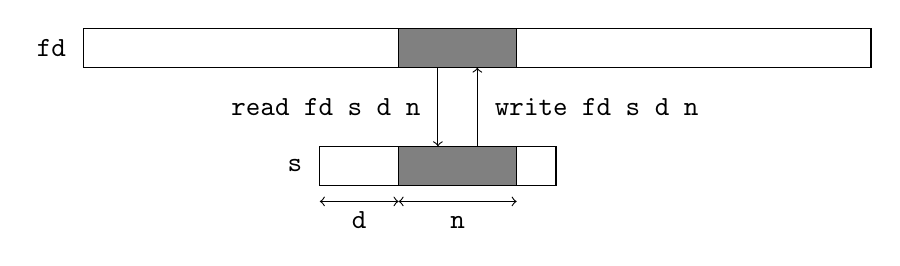
\begin{tikzpicture}[font={\ttfamily}]
\path[draw,fill=gray] (1,1.5) rectangle +(1.5, 0.5);
\path[draw] (-3,1.5) rectangle +(10, 0.5);
\node[anchor=east] at (-3.1,1.75) {fd};

\draw[->] (1.5, 1.5) to node [left=1mm] {read fd s d n} (1.5, 0.5);
\draw[<-] (2, 1.5) to node [right=1mm] {write fd s d n} (2, 0.5);

\path[draw,fill=gray] (1,0) rectangle +(1.5, 0.5);
\path[draw] (0,0) rectangle (3, 0.5);
\node[anchor=east] at (-0.1,0.25) {s};

\draw[<->] (0,-0.2) to node [below] {\phantom{n}d\phantom{n}} (1,-0.2);
\draw[<->] (1,-0.2) to node [below] {\phantom{d}n\phantom{d}} (2.5,-0.2);
\end{tikzpicture}
\end{myimage}
%
\ml+read+ and \ml+single_write+ return the number of bytes actually
read or written.

Reads and write calls are performed from the file descriptor's current
read/write position (if the file was opened in \ml+O_APPEND+ mode,
this position is set at the end of the file prior to any
write). After the system call, the current position is advanced by
the number of bytes read or written.

For writes, the number of bytes actually written is usually the number
of bytes requested. However there are exceptions: (i) if it is not
possible to write the bytes (\eg{} if the disk is full) (ii) the
descriptor is a pipe or a socket open in non-blocking mode (iii) due to
{\ocaml}, if the write is too large.

The reason for (iii) is that internally {\ocaml} uses auxiliary
buffers whose size is bounded by a maximal value. If this value is
exceeded the write will be partial. To work around this problem
{\ocaml} also provides the function \libvalue{Unix}{write} which
iterates the writes until all the data is written or an error occurs.
The problem is that in case of error there's no way to know the number
of bytes that were actually written. Hence \ml+single_write+ should be
preferred because it preserves the atomicity of writes (we know
exactly what was written) and it is more faithful to the original Unix
system call (note that the implementation of \ml+single_write+ is
described in section~\ref{single_write}).

%%% The french version has that here, but I don't think it belongs
%%% here.
%% In the following chapter, we shall see that when we write to a 
%% file descriptor which refers to a pipe or a lock file placed
%% in input/output blocking mode and which is then interrupted by a signal,
%% the call \ml+single_write+ returns an error \ml+EINTR+.
  
\begin{example} 
Assume \ml+fd+ is a descriptor open in write-only mode. 
%
\begin{lstlisting}
write fd "Hello world!" 3 7
\end{lstlisting}
%
writes the characters \ml+"lo worl"+ in the corresponding file,
and returns 7.
\end{example}

For reads, it is possible that the number bytes actually read is
smaller than the number of requested bytes. For example when the end
of file is near, that is when the number of bytes between the current
position and the end of file is less than the number of requested
bytes. In particular, when the current position is at the end of file,
\ml+read+ returns zero. The convention \quotes{zero equals end of
  file} also holds for special files, pipes and sockets. For example,
\ml+read+ on a terminal returns zero if we issue a \ml+ctrl-D+ on the
input.

Another example is when we read from a terminal. In that case,
\ml+read+ blocks until an entire line is available. If the line length
is smaller than the requested bytes \ml+read+ returns immediately with
the line without waiting for more data to reach the number of
requested bytes. (This is the default behavior for terminals, but it
can be changed to read character-by-character instead of
line-by-line, see section~\ref{sec/speciaux} and the type
\libtype{Unix}{terminal\_io} for more details.)

\begin{example} 
The following expression reads at most 100 characters from standard
input and returns them as a string.
%
\begin{lstlisting}
let buffer = String.create 100 in
let n = read stdin buffer 0 100 in
  String.sub buffer 0 n
\end{lstlisting}
\end{example}

\begin{example} 
The function \ml+really_read+ below has the same interface as
\ml+read+, but makes additional read attempts to try to get
the number of requested bytes. It raises the exception
\ml+End_of_file+ if the end of file is reached while doing this.
%
\begin{lstlisting}
let rec really_read fd buffer start length =
  if length <= 0 then () else
  match read fd buffer start length with
  | 0 -> raise End_of_file
  | r -> really_read fd buffer (start + r) (length - r);;
\end{lstlisting}
%
\end{example}

\section{Closing a descriptor}

The system call \syscall{close} closes a file descriptor.
%
\begin{listingcodefile}{tmpunix.mli}
val $\libvalue{Unix}{close}$ : file_descr -> unit
\end{listingcodefile}
% 

Once a descriptor is closed, all attempts to read, write, or do
anything else with the descriptor will fail. Descriptors should be
closed when they are no longer needed; but it is not mandatory. In
particular, and in contrast to \ml+Pervasives+'
channels, a file descriptor doesn't need to be closed to ensure that
all pending writes have been performed as write requests made with
\ml+write+ are immediately transmitted to the kernel. On the other
hand, the number of descriptors allocated by a process is limited by
the kernel (from several hundreds to thousands). Doing a \ml+close+ on
an unused descriptor releases it, so that the process does not run out
of descriptors.

\section{\label{ex/filecopy}Complete example: file copy}

We program a command \ml+file_copy+ which, given two arguments 
\ml+f1+ and \ml+f2+, copies to the file \ml+f2+ the bytes contained 
in \ml+f1+.
%
\begin{listingcodefile}{file_copy.ml}
open Unix;;

let buffer_size = 8192;;
let buffer = String.create buffer_size;;

let file_copy input_name output_name =
  let fd_in = openfile input_name [O_RDONLY] 0 in
  let fd_out = openfile output_name [O_WRONLY; O_CREAT; O_TRUNC] 0o666 in
  let rec copy_loop () = match read fd_in buffer 0 buffer_size with
    |  0 -> ()
    | r -> ignore (write fd_out buffer 0 r); copy_loop () 
  in
  copy_loop ();
  close fd_in;
  close fd_out;;
\end{listingcodefile}
%
\begin{codefile}{copy.ml}
open Unix
open File_copy
\end{codefile}
%
\begin{listingcodefile}{copy.ml}
let copy () =
  if Array.length Sys.argv = 3 then begin
    file_copy Sys.argv.(1) Sys.argv.(2);
    exit 0
  end else begin
    prerr_endline 
      ("Usage: " ^ Sys.argv.(0) ^ " <input_file> <output_file>");
    exit 1
  end;;

handle_unix_error copy ();;
\end{listingcodefile}
%

The bulk of the work is performed by the the function \ml+file_copy+.
First we open a descriptor in read-only mode on the input file and
another in write-only mode on the output file. 

If the output file already exists, it is truncated (option
\ml+O_TRUNC+) and if it does not exist it is created (option
\ml+O_CREAT+) with the permissions \ml+rw-rw-rw-+ modified by the creation
mask. (This is unsatisfactory: if we copy an executable file, we would
like the copy to be also executable. We will see later how to give
a copy the same permissions as the original.)

In the \ml+copy_loop+ function we do the copy by blocks of
\ml+buffer_size+ bytes. We request \ml+buffer_size+ bytes to read. If
\ml+read+ returns zero, we have reached the end of file and the copy
is over. Otherwise we write the \ml+r+ bytes we have read in the
output file and start again.

Finally, we close the two descriptors. The main program \ml+copy+
verifies that the command received two arguments and passes them to
the function \ml+file_copy+.

Any error occurring during the copy results in a \ml+Unix_error+
caught and displayed by \ml+handle_unix_error+. Example of errors
include inability to open the input file because it does not
exist, failure to read because of restricted permissions, failure to
write because the disk is full, \etc

\begin{exercise} 
Add an option \ml+-a+ to the program, such that 
\ml+file_copy -a f1 f2+ appends the contents of \ml+f1+ to the end of
the file \ml+f2+. 
\end{exercise}
\begin{answer}
If the option \ml+-a+ is supplied, we need to do 
%
\begin{lstlisting}
openfile output_name [O_WRONLY; O_CREAT; O_APPEND] 0o666
\end{lstlisting}
%
instead of
%
\begin{lstlisting}
openfile output_name [O_WRONLY; O_CREAT; O_TRUNC] 0o666
\end{lstlisting}
%
Parsing the new option from the command line is left to the reader. 
\end{answer}

\section{The cost of system calls and buffers}

In the example \ml+file_copy+, reads were made in blocks of 8192
bytes. Why not read byte per by byte, or megabyte per by megabyte?
The reason is efficiency.

Figure~\ref{fig/copy-speed} shows the copy speed of \ml+file_copy+, in
bytes per second, against the size of blocks (the value
\ml+buffer_size+). The amount of data transferred is the same
regardless of the size of the blocks.
\begin{myfigure}
\begin{myimage}[width="100\%"]
\begin{tikzpicture}[font=\tiny]
\pgfsetplotmarksize{0.8pt}
\draw plot[only marks,mark=*] file {data/speed-log.data};

% x-axis
\draw (0,-1) -- (7,-1);
\foreach \x in {0,...,7} { \draw (\x,-1) -- (\x,-0.95); };
\node at (0,-1.3) {\phantom{$^{2}$}1\phantom{$^{2}$}};
\node at (1,-1.3) {\phantom{$^{2}$}10\phantom{$^{2}$}};
\node at (2,-1.3) {\phantom{$^{2}$}100\phantom{$^{2}$}};
\foreach \x in {3,...,7} { \node at (\x,-1.3) {\phantom{$^{\x}$}10$^\x$}; };
\node at (8.5, -1.3) {Size (bytes)\phantom{1$^{1}$}};

% y-axis
\draw (-0.5,-0.5) -- (-0.5, 2.5);
\foreach \y in {-1,...,3} { \draw (-0.5,\y) -- (-0.45,\y); };
\node[anchor=east] at (-0.5,-1) {0.1\phantom{$^{3}$}};
\node[anchor=east] at (-0.5,0) {1\phantom{$^{3}$}};
\node[anchor=east] at (-0.5,1) {10\phantom{$^{3}$}};
\node[anchor=east] at (-0.5,2) {100\phantom{$^{3}$}};
\node[anchor=east] at (-0.5,3) {10$^{3}$};

\node[anchor=east] at (-0.5,3.5) {Speed (MB/s)};
\end{tikzpicture}
\end{myimage}
\caption{Copy speed as a function of block size}
\label{fig/copy-speed}
\end{myfigure}
For small block sizes, the copy speed is almost proportional to the
block size. Most of the time is spent not in data transfers but in the
execution of the loop \ml+copy_loop+ and in the calls to \ml+read+ and
\ml+write+. By profiling more carefully we can see that most of the
time is spent in the calls to \ml+read+ and \ml+write+. We conclude
that a system call, even if it has not much to do, takes a minimum of
about 4 micro-seconds (on the machine that was used for the test~---~a
2.8 GHz Pentium 4 ), let us say from 1 to 10 microseconds.  For small
input/output blocks, the duration of the system call dominates.
  
For larger blocks, between 4KB and 1MB, the copy speed is constant and
maximal. Here, the time spent in system calls and the loop is small
relative to the time spent on the data transfer. Also, the buffer
size becomes bigger than the cache sizes used by the system and the
time spent by the system to make the transfer dominates the cost of a
system call\footnote{In fact, {\ocaml} limits the size of data
  transfers to 16KB (in the current version) and repeats \ml+write+
  system calls to make the complete transfer~---~see the discussion in
  section~\ref{single_write}. But this limit is bigger than the
  size of system caches and it is not observable.}.

Finally, for very large blocks (8MB and more) the speed is slightly
under the maximum.  Coming into play here is the time needed to
allocate the block and assign memory pages to it as it fills up.

\begin{codefile}{speed_write.c}
#include <errno.h>
#include <string.h>
#include <caml/mlvalues.h>
#include <caml/memory.h>
#include <caml/signals.h>
#include <caml/unixsupport.h>

#define LONG_BUFFER_SIZE 9388608

CAMLprim value speed_write
        (value fd, value buf, value ofs, value len) {
  CAMLparam4(fd, buf, ofs, len);
  long numbytes;
  int ret = 0;
  char iobuf[LONG_BUFFER_SIZE];
  numbytes = Long_val(len);
  if (numbytes > LONG_BUFFER_SIZE) numbytes = LONG_BUFFER_SIZE;
  /* memmove (iobuf, &Byte(buf, Long_val(ofs)), numbytes); */
  /* enter_blocking_section (); */
  /* ret = write(Int_val(fd), iobuf, (int) numbytes); */
  ret = write(Int_val(fd), &Byte(buf, Long_val(ofs)), (int) numbytes);
  /* leave_blocking_section (); */
  if (ret == -1) uerror("write", Nothing);
  CAMLreturn (Val_int(ret));
}
\end{codefile}
%
\begin{codefile}{speed.ed}
f speed.ml
r file_copy.ml
3a
external speed_write :
   file_descr -> string -> int -> int -> int = "speed_write";;
.
/buffer_size/,/file_copy/c
let file_copy buffer_size input_name output_name =
  let buffer = String.create buffer_size in
.
/write/s/write/speed_write/
$a

let rec power n k = if k > 0 then n * power n (pred k) else 1;;
let copy () =
  if Array.length Sys.argv = 2 then begin
    let file = Sys.argv.(1) in
    let tmp = Filename.temp_file "foo" "bar" in
    let mega_octets = float (10 * (lstat file).st_size) /. 1e6 in
    (* put file in cache *)
    file_copy 10 file "/dev/null";
    for i = 23 downto 0 do 
      let start = let t = Unix.times () in t.tms_utime +. t.tms_stime in
      let block = power 2 i in
      for i = 1 to 10 do file_copy block file tmp done;
      let stop = let t = Unix.times () in t.tms_utime +. t.tms_stime in
      let time = stop -. start in
      let speed = mega_octets /. time in
      Printf.printf "%9d %.2f" block speed; 
      print_newline ();
    done;
      exit 0
  end else begin
    prerr_endline ("Usage: " ^Sys.argv.(0)^ " <input_file> <output_file>");
    exit 1
  end;;

handle_unix_error copy ();;
.
wq
\end{codefile}
% $

The moral of the story is that, a system call, even if it does very little work,
costs dearly~---~much more than a normal function call: roughly, 2 to
20 microseconds for each system call, depending on the
architecture. It is therefore important to minimize the number of
system calls. In particular, read and write operations should be made
in blocks of reasonable size and not character by character.

In examples like \ml+file_copy+, it is not difficult to do
input/output with large blocks. But other types of programs are more
naturally written with character by character input or output (\eg{}
reading a line from a file, lexical analysis, displaying a number \etc).
To satisfy the needs of these programs, most systems provide
input/output libraries with an additional layer of software between
the application and the operating system. For example, in {\ocaml} the
\ml+Pervasives+ module defines the abstract types
\libtype{Pervasives}{in\_channel} and
\libtype{Pervasives}{out\_channel}, similar to file descriptors, and
functions on these types like \libvalue{Pervasives}{input\_char},
\libvalue{Pervasives}{input\_line},
\libvalue{Pervasives}{output\_char}, or
\libvalue{Pervasives}{output\_string}.  This layer uses buffers to
group sequences of character by character reads or writes into a
single system call to read or write. This results in better
performance for programs that proceed character by character.
Moreover this additional layer makes programs more portable: we just
need to implement this layer with the system calls provided by another
operating system to port all the programs that use this library on
this new platform.

\section{Complete example: a small input/output library}

To illustrate the buffered input/output techniques, we implement a fragment
of {\ocaml} \ml+Pervasives+ library. Here is the interface:
%
\begin{listingcodefile}{io.mli}
exception End_of_file

type in_channel
val open_in : string -> in_channel
val input_char : in_channel -> char
val close_in : in_channel -> unit

type out_channel
val open_out : string -> out_channel
val output_char : out_channel -> char -> unit
val close_out : out_channel -> unit
\end{listingcodefile}
%
We start with the \quotes{input} part. The abstract type 
\ml+in_channel+ is defined as follows: 
%
\begin{listingcodefile}{io.ml}
open Unix;;

type in_channel =
  { in_buffer: string;
    in_fd: file_descr;
    mutable in_pos: int;
    mutable in_end: int };;
exception End_of_file
\end{listingcodefile}
%
The character string of the \ml+in_buffer+ field is, literally, the
buffer.  The field \ml+in_fd+ is a (Unix) file descriptor, opened on
the file to read. The field \ml+in_pos+ is the current read position
in the buffer.  The field \ml+in_end+ is the number of valid
characters preloaded in the buffer.
%
\begin{myimage}[width="85\%"]
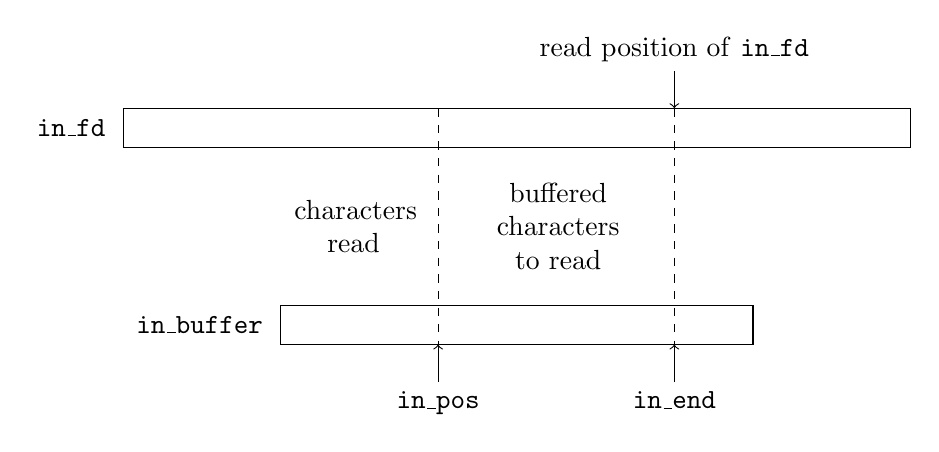
\begin{tikzpicture}
\path[draw] (-3,2.5) rectangle +(10, 0.5);
\node[anchor=east] at (-3.1,2.75) {\texttt{in\_fd}};
\draw[dashed] (1,3) to node [left=2mm,text width=1.5cm,text centered] 
 {characters read} (1,0);

\draw[dashed] (4,3) to node [left=1mm,text width=2.5cm,text centered] 
 {buffered characters to read} (4,0);

\path[draw] (-1,0) rectangle +(6, 0.5);
\node[anchor=east] at (-1.1,0.25) {\texttt{in\_buffer}};

\node (fdpos) at (4,3.75) {read position of \texttt{in\_fd}};
\draw[->] (fdpos.south) to (4,3);

\node (ipos) at (1,-0.75) {\texttt{\phantom{d}in\_pos\phantom{d}}};
\node (iend) at (4,-0.75) {\texttt{\phantom{p}in\_end\phantom{p}}};
\draw[->] (ipos.north) to (1,0);
\draw[->] (iend.north) to (4,0);
\end{tikzpicture}
\end{myimage}
The fields \ml+in_pos+ and \ml+in_end+ will be modified in place during 
read operations; we therefore declare them as \ml+mutable+.
%
\begin{listingcodefile}{io.ml}
let buffer_size = 8192;;
let open_in filename =
  { in_buffer = String.create buffer_size;
    in_fd = openfile filename [O_RDONLY] 0;
    in_pos = 0;
    in_end = 0 };;
\end{listingcodefile}
%
When we open a file for reading, we create a buffer of reasonable size
(large enough so as not to make too many system calls; small enough so
as not to waste memory). We then initialize the field \ml+in_fd+ with
a Unix file descriptor opened in read-only mode on the given file. The
buffer is initially empty (it does not contain any character from the
file); the field \ml+in_end+ is therefore initialized to zero.
%
\begin{listingcodefile}{io.ml}
let input_char chan =
  if chan.in_pos < chan.in_end then begin
    let c =  chan.in_buffer.[chan.in_pos] in
      chan.in_pos <- chan.in_pos + 1;
      c
  end else begin
    match read chan.in_fd chan.in_buffer 0 buffer_size
    with 0 -> raise End_of_file
       | r -> chan.in_end <- r;
              chan.in_pos <- 1;
              chan.in_buffer.[0]
  end;;
\end{listingcodefile}
% 
To read a character from an \ml+in_channel+, we do one of two
things.  Either there is at least one unread character in the buffer;
that is to say, the field \ml+in_pos+ is less than the field
\ml+in_end+. We then return this character located at \ml+in_pos+, and
increment \ml+in_pos+. Or the buffer is empty and we call \ml+read+ to
refill the buffer. If \ml+read+ returns zero, we have reached the end
of the file and we raise the exception \ml+End_of_file+. Otherwise, we
put the number of characters read in the field \ml+in_end+ (we may
receive less characters than we requested, thus the buffer may be
only partially refilled) and we return the first character read.
%
\begin{listingcodefile}{io.ml}
let close_in chan =
  close chan.in_fd;;
\end{listingcodefile}
%
Closing an \ml+in_channel+ just closes the underlying Unix file descriptor. 

The \quotes{output} part is very similar to the \quotes{input}
part. The only asymmetry is that the buffer now contains incomplete
writes (characters that have already been buffered but not written to
the file descriptor), and not reads in advance (characters that have
buffered, but not yet read).

\begin{myimage}[width="85\%"]
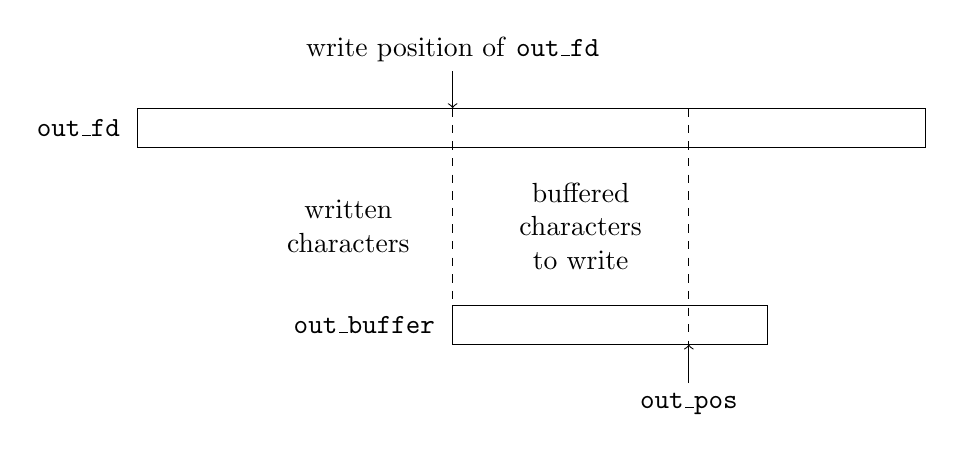
\begin{tikzpicture}
\path[draw] (-3,2.5) rectangle +(10, 0.5);
\node[anchor=east] at (-3.1,2.75) {\texttt{out\_fd}};
\draw[dashed] (1,3) to node [left=2mm,text width=2cm,text centered] 
 {written characters} (1,0);

\draw[dashed] (4,3) to node [left,text width=2.5cm,text centered] 
 {buffered characters to write} (4,0);

\path[draw] (1,0) rectangle +(4, 0.5);
\node[anchor=east] at (0.9,0.25) {\texttt{out\_buffer}};

\node (fdpos) at (1,3.75) {write position of \texttt{out\_fd}};
\draw[->] (fdpos.south) to (1,3);

\node (opos) at (4,-0.75) {\texttt{out\_pos}};
\draw[->] (opos.north) to (4,0);
\end{tikzpicture}
\end{myimage}
%
\begin{listingcodefile}{io.ml}
type out_channel =
  { out_buffer: string;
    out_fd: file_descr;
    mutable out_pos: int };;

let open_out filename =
  { out_buffer = String.create 8192;
    out_fd = openfile filename [O_WRONLY; O_TRUNC; O_CREAT] 0o666;
    out_pos = 0 };;

let output_char chan c =
  if chan.out_pos < String.length chan.out_buffer then begin
    chan.out_buffer.[chan.out_pos] <- c;
    chan.out_pos <- chan.out_pos + 1
  end else begin
    ignore (write chan.out_fd chan.out_buffer 0 chan.out_pos);
    chan.out_buffer.[0] <- c;
    chan.out_pos <- 1
  end;;

let close_out chan =
  ignore (write chan.out_fd chan.out_buffer 0 chan.out_pos);
  close chan.out_fd;;
\end{listingcodefile}
% 
To write a character on an \ml+out_channel+, we do one of two things.
Either the buffer is not full and we just store the character in the
buffer at the position \ml+out_pos+ and increment that value. Or the
buffer is full and we empty it with a call to \ml+write+ and then
store the character at the beginning of the buffer.
 
When we close an \ml+out_channel+, we must not forget to write the
buffer contents (the characters from 0 to \ml+out_pos - 1+) to the
file otherwise the writes made on the channel since the last time
the buffer was emptied would be lost.

\begin{exercise} 
Implement the function:
%
\begin{lstlisting}
val output_string : out_channel -> string -> unit
\end{lstlisting}
%
which behaves like a sequence of \ml+output_char+ on each 
character of the string, but is more efficient.
\enlargethispage{2\baselineskip} %% To avoid a widow
\end{exercise}
\begin{answer}
The idea is to copy the string to output into the buffer. We need to
take into account the case where there is not enough space in the
buffer (in that case the buffer needs to emptied), and also the case
where the string is longer than the buffer (in that case it can 
be written directly). Here is a possible solution.
%
\begin{codefile}{ex2.ml}
open Unix;;
\end{codefile}
%
\begin{listingcodefile}{ex2.ml}
let output_string chan s =
  let avail = String.length chan.out_buffer - chan.out_pos in
  if String.length s <= avail then begin
    String.blit s 0 chan.out_buffer chan.out_pos (String.length s);
    chan.out_pos <- chan.out_pos + String.length s
  end
  else if chan.out_pos = 0 then begin
    ignore (write chan.out_fd s 0 (String.length s))
  end
  else begin
    String.blit s 0 chan.out_buffer chan.out_pos avail;
    let out_buffer_size = String.length chan.out_buffer in
    ignore (write chan.out_fd chan.out_buffer 0 out_buffer_size);
    let remaining = String.length s - avail in
    if remaining < out_buffer_size then begin
      String.blit s avail chan.out_buffer 0 remaining;
      chan.out_pos <- remaining
    end else begin
      ignore (write chan.out_fd s avail remaining);
      chan.out_pos <- 0
    end
  end;;
\end{listingcodefile}
%
\begin{codefile}{ex2.ml}
let ex2 () = 
  if Array.length Sys.argv < 3 then begin 
     prerr_string "Usage: test <sources> <dest>"; 
     exit 2;
  end;
  let fdin = open_in Sys.argv.(1) in
  let fdout = open_out Sys.argv.(2) in
  prerr_endline "copying";
  try while true do output_char fdout (input_char fdin) done
  with End_of_file -> 
   prerr_endline "Done";
   output_string fdout "The end.\n";
   prerr_endline "Closing";
   close_out fdout;;

handle_unix_error ex2 ();;
\end{codefile}
%
\begin{codefile}{ex2.test}
./ex2.byte ex2.ml ex2.out
(cat ex2.ml; echo "C'est la fin.") | diff --brief - ex2.out
rm ex2.out
\end{codefile}
\end{answer}


\section{Positioning}

The system call \syscall{lseek} allows to set the current read/write
position of a file descriptor.
%
\begin{codefile}{tmpunix.mli}
type seek_command = Unix.seek_command
\end{codefile}
%
\begin{listingcodefile}{tmpunix.mli}
val $\libvalue{Unix}{lseek}$ : file_descr -> int -> seek_command -> int
\end{listingcodefile}
%
The first argument is the file descriptor and the second one the
desired position. The latter is interpreted according to the value
of the third argument of type \libtype{Unix}{seek\_command}. This
enumerated type specifies the kind of position:
%
\begin{mltypecases}
\begin{tabular}{@{}lp{0.8\textwidth}}
\ml+SEEK_SET+ & Absolute position. The second argument specifies
the character number to point to. The first character of a file is at
position zero.\\
%
\ml+SEEK_CUR+ & Position relative to the current position. 
The second argument is an offset relative to the  
current position. A positive value moves forward and a negative value
moves backwards.\\
%
\ml+SEEK_END+ & Position relative to the end of file. The 
second argument is an offset relative to the end of file.
As for \ml+SEEK_CUR+, the offset may be positive or negative.
\end{tabular}
\end{mltypecases}
% 
The value returned by \ml+lseek+ is the resulting absolute
read/write position.

An error is raised if a negative absolute position is
requested. The requested position can be located after the end
of file. In that case, a \ml+read+ returns zero (end of
file reached) and a \ml+write+ extends the file with zeros until 
that position and then writes the supplied data.

\begin{example} 
To position the cursor on the 1000th character of a file:
%
\begin{lstlisting}
lseek fd 1000 SEEK_SET
\end{lstlisting}
%
To rewind by one character:
%
\begin{lstlisting}
lseek fd (-1) SEEK_CUR
\end{lstlisting}
%
To find out the size of a file:
%
\begin{lstlisting}
let file_size = lseek fd 0 SEEK_END in ...
\end{lstlisting}
\end{example}

For descriptors opened in \ml+O_APPEND+ mode, the read/write position
is automatically set at the end of the file before each write.  Thus
a call \ml+lseek+ is useless to set the write position, it may however
be useful to set the read position. 

The behavior of \ml+lseek+ is undefined on certain type of files for
which absolute access is meaningless: communication devices (pipes,
sockets) but also many special files like the terminal.
In most Unix implementations a call to \ml+lseek+ on these files is
simply ignored: the read/write position is set but read/write
operations ignore it. In some implementations, \ml+lseek+ on a pipe or
a socket triggers an error.

\begin{exercise}
The command \ml+tail+ displays the last $n$ lines of a file.
How can it be implemented efficiently on regular files? What can we 
do for the other kind of files? How can the option \ml+-f+ be
implemented (cf. \ml+man tail+)?
\enlargethispage{3\baselineskip} %% To avoid a widow
\end{exercise}
\begin{answer}
A naive implementation of \ml+tail+ is to read the file sequentially
from the beginning, keeping the last $n$ lines read in a circular
buffer. When we reach the end of file, we display the buffer.
When the data comes from a pipe or a special file which
does not implement \ml+lseek+, there is no better way.

However if the data is coming from a normal file, it is better to read
the file from the end. With \ml+lseek+, we read the last 4096
characters. We scan them for the end of lines. If there are at least
$n$ of them, we output and display the corresponding lines.
Otherwise, we start again by adding the next preceding 4096
characters, \etc

To add the option \ml+-f+, we first proceed as above and then we go
back at the end of the file and try to \ml+read+ from there. If
\ml+read+ returns data we display it immediately and start again. If it
returns \ml+0+ we wait some time (\ml+sleep 1+) and try again.
\end{answer}

\section{Operations specific to certain file types}

In Unix, data communication is done via file descriptors representing
either permanent files (files, peripherals) or volatile ones (pipes
and sockets, see chapters~\ref{sec/pipes} and \ref{sec/sockets}). File
descriptors provide a uniform and media-independent interface for data
communication. Of course the actual implementation of the operations
on a file descriptor depends on the underlying media.

However this uniformity breaks when we need to access all the
features provided by a given media. General operations (opening,
writing, reading, \etc) remain uniform on most descriptors but even,
on certain special files, these may have an ad hoc behavior defined
by the kind of peripheral and its parameters. There are also
operations that work only with certain kind of media.

\subsection*{Normal files}

We can shorten a normal file with the system calls
\syscall{truncate} and \syscall{ftruncate}.
%
\begin{listingcodefile}{tmpunix.mli}
val $\libvalue{Unix}{truncate}$  : string -> int -> unit
val $\libvalue{Unix}{ftruncate}$ : file_descr -> int -> unit
\end{listingcodefile}
%
The first argument is the file to truncate and the second the desired
size. All the data after this position is lost.

\subsection*{Symbolic links}

Most operations on files \quotes{follow} symbolic links in the sense
that they do not apply to the link itself but to the file on which the
link points (for example \indexvalue{openfile},
\indexvalue{stat}, \indexvalue{truncate}, \indexvalue{opendir}, \etc). 

The two system calls \syscall{symlink} and \syscall{readlink} operate
specifically on symbolic links:
%
\begin{listingcodefile}{tmpunix.mli}
val $\libvalue{Unix}{symlink}$  : string -> string -> unit
val $\libvalue{Unix}{readlink}$ : string -> string
\end{listingcodefile}
% 
The call \ml+symlink f1 f2+ creates the file \ml+f2+ as a symbolic
link to \ml+f1+ (like the Unix command \ml+ln -s f1 f2+). The call
\ml+readlink+ returns the content of a symbolic link, \ie{} the name of
the file to which the link points.

\subsection*{\label{sec/speciaux}Special files}

Special files can be of \quotes{character} or \quotes{block} type.
The former are character streams: we can read or write characters only
sequentially. These are the terminals, sound devices, printers, \etc{}
The latter, typically disks, have a permanent medium: characters can
be read by blocks and even seeked relative to the current position.

Among the special files, we may distinguish:
\begin{mltypecases}
\begin{tabular}{@{}lp{0.8\textwidth}}
\ml+/dev/null+ & This is the black hole which swallows
  everything we put into and from which nothing comes out. This is
  extremely useful for ignoring the results of a process: we redirect
  its output to \ml+/dev/null+ (see chapter~\ref{sec/pipes}).\\
%
\ml+/dev/tty*+ & These are the control terminals. \\
%
\ml+/dev/pty*+ & These are the pseudo-terminals: they are not real
  terminals but simulate them (they provide the same interface). \\
%
\ml+/dev/hd*+ & These are the disks. \\
%
\ml+/proc+ & Under Linux, system parameters organized as a
  file system. They allow reads and writes.
\end{tabular}
\end{mltypecases}

The usual file system calls on special files can behave differently.
However, most special files (terminals, tape drives, disks, \etc)
respond to \ml+read+ and \ml+write+ in the obvious manner (but
sometimes with restrictions on the number of bytes written or read),
but many ignore \indexvalue{lseek}.

In addition to the usual file system calls, special files which
represent peripherals must be commanded and/or configured
dynamically. For example, for a tape drive, rewind or fast forward the
tape; for a terminal, choice of the line editing mode, behavior of
special characters, serial connection parameters (speed, parity,
\etc).  These operations are made in Unix with the system call
\syscall{ioctl} which group together all the particular
cases. However, this system call is not provided by {\ocaml}; it is
ill-defined and cannot be treated in a uniform way.

\subsection*{\label{sec/termio}Terminals}

Terminals and pseudo-terminals are special files of type character
which can be configured from {\ocaml}. The system call
\syscall{tcgetattr} takes a file descriptor open on a special file
and returns a structure of type \libtype{Unix}{terminal\_io} which
describes the status of the terminal according to the \textsc{posix} 
standard.
%
\begin{codefile}{tmpunix.mli}
type terminal_io = Unix.terminal_io
\end{codefile}
%
\begin{lstlisting}
type $\libtype{Unix}{terminal\_io}$ = 
  { c_ignbrk : bool; c_brk_int : bool; ...;  c_vstop : char }
\end{lstlisting}
%
\begin{listingcodefile}{tmpunix.mli}
val $\libvalue{Unix}{tcgetattr}$ : file_descr -> terminal_io
\end{listingcodefile}
%
This structure can be modified and given to the function 
\syscall{tcsetattr} to change the attributes of the peripheral.
%
\begin{codefile}{tmpunix.mli}
type setattr_when = Unix.setattr_when
\end{codefile}
%
\begin{listingcodefile}{tmpunix.mli}
val $\libvalue{Unix}{tcsetattr}$ : file_descr -> setattr_when -> terminal_io -> unit
\end{listingcodefile}
% 

The first argument is the file descriptor of the peripheral. The last
argument is a structure of type \ml+terminal_io+ describing the
parameters of the peripheral as we want them. The second argument is a
value of the enumerated type \libtype{Unix}{setattr\_when} that
indicates when the change must be done: immediately (\ml+TCSANOW+),
after having transmitted all written data (\ml+TCSADRAIN+) or after
having read all the received data (\ml+TCAFLUSH+). \ml+TCSADRAIN+ is
recommended for changing write parameters and \ml+TCSAFLUSH+ for read
parameters.

\begin{example}
When a password is read, characters entered by the user should not be
echoed if the standard input is connected to a terminal or a
pseudo-terminal.
%
\begin{codefile}{passwd.ml}
open Unix;;
\end{codefile}
%
\begin{listingcodefile}{passwd.ml}
let read_passwd message = 
  match
    try 
      let default = tcgetattr stdin in
      let silent = 
        { default with 
          c_echo = false; 
          c_echoe = false; 
          c_echok = false; 
          c_echonl = false; 
        } in
      Some (default, silent) 
    with _ -> None
  with 
  | None -> input_line Pervasives.stdin
  | Some (default, silent) -> 
      print_string message; 
      flush Pervasives.stdout;
      tcsetattr stdin TCSANOW silent;
      try 
        let s = input_line Pervasives.stdin in 
        tcsetattr stdin TCSANOW default; s
      with x -> 
        tcsetattr stdin TCSANOW default; raise x;;
\end{listingcodefile}
% 
The \ml+read_passwd+ function starts by getting the current settings
of the terminal connected to \ml+stdin+. Then it defines a modified
version of these in which characters are not echoed. If this fails the
standard input is not a control terminal and we just read a
line. Otherwise we display a message, change the terminal settings, read the
password and put the terminal back in its initial state. Care must be
taken to set the terminal back to its initial state even after a read
failure.
\end{example}
% 
Sometimes a program needs to start another and connect its standard input
to a terminal (or pseudo-terminal). {\ocaml} does not provide any
support for this\footnote {The Cash library~\cite {Cash} supplies
  such functions.}. To achieve that, we must manually look among the
pseudo-terminals (in general, they are files with names in the form of
\ml+/dev/tty[a-z][a-f0-9]+) and find one that is not already open. We
can then open this file and start the program with this file on its
standard input.

Four other functions control the stream of data of a terminal
(flush waiting data, wait for the end of transmission and restart
communication).
%
\begin{listingcodefile}{tmpunix.mli}
val $\libvalue{Unix}{tcsendbreak}$ : file_descr -> int -> unit
\end{listingcodefile}
%
The function \syscall{tcsendbreak} sends an interrupt to the 
peripheral. The second argument is the duration of the interrupt
(\ml+0+ is interpreted as the default value for the 
peripheral).
%
\begin{listingcodefile}{tmpunix.mli}
val $\libvalue{Unix}{tcdrain}$ : file_descr -> unit
\end{listingcodefile}
%
The function \syscall{tcdrain} waits for all written data to
be transmitted.
%
\begin{codefile}{tmpunix.mli}
type flush_queue = Unix.flush_queue
\end{codefile}
%
\begin{listingcodefile}{tmpunix.mli}
val $\libvalue{Unix}{tcflush}$ : file_descr -> flush_queue -> unit
\end{listingcodefile}
% 
Depending on the value of the second argument, a call to the
function \syscall{tcflush} discards the data written but not yet
transmitted (\ml+TCIFLUSH+), or the data received but not yet read
(\ml+TCOFLUSH+) or both (\ml+TCIOFLUSH+).
%
\begin{codefile}{tmpunix.mli}
type flow_action = Unix.flow_action
\end{codefile}
%
\begin{listingcodefile}{tmpunix.mli}
val $\libvalue{Unix}{tcflow}$ : file_descr -> flow_action -> unit
\end{listingcodefile}
% 
Depending on the value of the second argument, a call to the
function \syscall{tcflow} suspends the data transmission
(\ml+TCOOFF+), restarts the transmission (\ml+TCOON+), sends a control
character \textsc{stop} or \textsc{start} to request the
transmission to be suspended (\ml+TCIOFF+) or restarted (\ml+TCION+).
%
\begin{listingcodefile}{tmpunix.mli}
val $\libvalue{Unix}{setsid}$ : unit -> int
\end{listingcodefile}
%
The function \syscall{setsid} puts the process in a new
session and detaches it from the terminal.

\section{Locks on files}

Two processes can modify the same file in parallel; however, their
writes may collide and result in inconsistent data. In some cases data
is always written at the end and opening the file with \ml+O_APPEND+
prevents this. This is fine for \ml+log+ files but it does not
work for files that store, for example, a database because writes are
performed at arbitrary positions. In that case processes using the
file must collaborate in order not to step on each others toes.  A
lock on the whole file can be implemented with an auxiliary file (see
page \pageref{page/lock}) but the system call \syscall{lockf} allows
for finer synchronization patterns by locking only parts of a file.
%
\begin{codefile}{tmpunix.mli}
type lock_command = Unix.lock_command
\end{codefile}
%
\begin{listingcodefile}{tmpunix.mli}
 val $\libvalue{Unix}{lockf}$ : file_descr -> lock_command -> int -> unit
\end{listingcodefile}


\section{\label{sec/copyrec}Complete example: recursive copy of files}

We extend the function \ml+file_copy+ (section~\ref{ex/filecopy}) to
support symbolic links and directories in addition to normal files.
For directories, we recursively copy their contents.

To copy normal files we reuse the function \ml+file_copy+ we already
defined.
\begin{lstlisting}
open Unix
...
let file_copy input_name output_name =
...
\end{lstlisting}
The function \ml+set_infos+ below modifies the owner, the  
access rights and the last dates of access/modification
of a file. We use it to preserve this information for copied files.
%
\begin{codefile}{copy_rec.ml}
open Unix;;
open File_copy;;
\end{codefile}
%
\begin{listingcodefile}{copy_rec.ml}
let set_infos filename infos =
  utimes filename infos.st_atime infos.st_mtime;
  chmod filename infos.st_perm;
  try
    chown filename infos.st_uid infos.st_gid
  with Unix_error(EPERM,_,_) -> ()
\end{listingcodefile}
%
The system call \syscall{utime} modifies the dates of access and 
modification.  We use \ml+chmod+ and \ml+chown+ to re-establish 
the access rights and the owner. For normal users, there are  
a certain number of cases where  \ml+chown+ will fail with a
\quotes{permission denied} error. We catch this error and ignore it.

Here's the main recursive function. 
\begin{listingcodefile}{copy_rec.ml}
let rec copy_rec source dest =
  let infos = lstat source in
  match infos.st_kind with
  | S_REG ->
      file_copy source dest;
      set_infos dest infos
  | S_LNK ->
      let link = readlink source in
      symlink link dest
  | S_DIR ->
      mkdir dest 0o200;
      Misc.iter_dir
        (fun file ->
          if file <> Filename.current_dir_name 
              && file <> Filename.parent_dir_name 
          then 
            copy_rec
              (Filename.concat source file)
              (Filename.concat dest file))
        source;
      set_infos dest infos
  | _ ->
      prerr_endline ("Can't cope with special file " ^ source)
\end{listingcodefile}
%
We begin by reading the information of the \ml+source+ file. If it is
a normal file, we copy its contents with \ml+file_copy+ and its
information with \ml+set_infos+. If it is a symbolic link, we read
where it points to and create a link pointing to the same object.  If
it is a directory, we create a destination directory, then we read the
directory's entries (ignoring the entries about the directory itself
or its parent) and recursively call \ml+copy_rec+ for each entry. All
other file types are ignored, with a warning.

The main program is straightforward:
%
\begin{codefile}{copyrec.ml}
open Unix
open Copy_rec
\end{codefile}
%
\begin{listingcodefile}{copyrec.ml}
let copyrec () =
  if Array.length Sys.argv <> 3 then begin
    prerr_endline ("Usage: " ^Sys.argv.(0)^ " <source> <destination>");
    exit 2
  end else begin
    copy_rec Sys.argv.(1) Sys.argv.(2);
    exit 0
  end
;;
handle_unix_error copyrec ();;
\end{listingcodefile}

\begin{exercise} 
\label{ex/copyrec}
Copy hard links cleverly. As written above \ml+copy_rec+ creates $n$
duplicates of the same file whenever a file occurs under $n$ different
names in the hierarchy to copy. Try to detect this situation, copy
the file only once and make hard links in the destination hierarchy.
\end{exercise}

\begin{answer}
For the files that have already been copied we keep a map from their
identity \ml+(st_dev, st_ino)+ to their destination file name. Before
each copy we consult the map to see if a file with the same identity
was already copied. If that's the case we do a hard link on the
destination file name instead of redoing the copy. To minimize the
size of the map we remember only the files which have more than one
name, \ie{} those for which \ml+st_nlink > 1+.
%
\begin{codefile}{copyrec_ex.ml}
open File_copy
open Copy_rec
open Sys
open Unix
\end{codefile}
%
\begin{listingcodefile}{copyrec_ex.ml}
let copied_files = (Hashtbl.create 53 : ((int * int), string) Hashtbl.t)

let rec copy source dest =
  let infos = lstat source in
  match infos.st_kind with
    S_REG ->
      if infos.st_nlink > 1 then begin
        try
          let dest' = 
            Hashtbl.find copied_files (infos.st_dev, infos.st_ino)
          in link dest' dest
        with Not_found ->
          Hashtbl.add copied_files (infos.st_dev, infos.st_ino) dest;
          file_copy source dest;
          set_infos dest infos
      end else begin
        file_copy source dest;
        set_infos dest infos
      end
\end{listingcodefile}
\begin{lstlisting}
  | S_LNK -> ...
\end{lstlisting}
\begin{codefile}{copyrec_ex.ml}
| _ -> ()
\end{codefile}
\end{answer}

\section{Complete example: {\normalfont\texttt{T}}ape {\normalfont\texttt{AR}}chive}

The \ml+tar+ file format (for \ml+t+ape \ml+ar+chive) can store a file
hierarchy into a single file. It can be seen as a mini file system.

In this section we define functions to read and write \ml+tar+
files. We also program a command \ml+readtar+ such that \ml+readtar a+
displays the name of the files contained in the archive \ml+a+ and
\ml+readtar a f+ extracts the contents of the file \ml+f+ contained in
\ml+a+. Extracting the whole file hierarchy of an archive and
generating an archive for a file hierarchy is left as an exercise.

\paragraph{File format specification}

A \ml+tar+ archive is a set of records. Each record represents a
file; it starts with a header which encodes the information
about the file (its name, type, size, owners, \etc) and is followed by 
the contents of the file. The header is a block of 512 bytes structured as
shown in table~\ref{fig/tar}.

\begin{mytable}
\begin{tabular}{rrlll}
Offset & Length & Code Type & Name & Description \\
\hline
  0&   100 & string  &  \ml+name+   & File name \\
100&     8 & octal   &  \ml+perm+   & File permissions\\
108&     8 & octal   &  \ml+uid+    & Id of user owner\\
116&     8 & octal   &  \ml+gid+    & Id of group owner\\
124&    12 & octal   &  \ml+size+   & File size (in bytes)\\
136&    12 & octal   &  \ml+mtime+  & Date of last modification\\
148&     8 & octal   &  \ml+checksum+ & Header checksum \\
156&     1 &character&  \ml+kind+   & File type  \\
157&   100 & octal   &  \ml+link+   & Link\\
257&     8 & string  &  \ml+magic+  & Signature (\ml+"ustar\032\032\0"+)\\
265&    32 & string  &  \ml+user+   & Name of user owner\\
297&    32 & string  &  \ml+group+  & Name of group owner\\
329&     8 & octal   &  \ml+major+  & Peripheral major number\\
337&     8 & octal   &  \ml+minor+  & Peripheral minor number\\
345&   167 &         &              & Padding \smallskip\\
\hline 
\end{tabular}
\begin{flushleft}
\small\textbf{Note.}\quad Field lengths are in number of
bytes. All fields are encoded with character strings terminated with
the null character \ml+'\000'+; except the fields \ml+kind+ and
\ml+size+ in which \ml+'\000'+ optional.
\end{flushleft}
\ifnothtml{\vspace{-\onelineskip}}
\caption {Header structure}
\label{fig/tar}
\end{mytable}
The file contents is stored right after the header, its size is
rounded to a multiple of 512 bytes (the extra space is filled with
zeros). Records are stored one after the other. If needed, the file is
padded with empty blocks to reach at least 20 blocks.

Since tar archives are also designed to be written on brittle media
and reread many years later, the header contains a \ml+checksum+
field which allows to detect when the header is damaged. Its value is
the sum of all the bytes of the header (to compute that sum we assume
that the \ml+checksum+ field itself is made of zeros).

The \ml+kind+ header field encodes the file type in a byte as follows\footnote {This field can 
  also take different values to encode
  pathological cases, for example when the value of a field exceeds
  its size or in extensions of the
  \ml+tar+ format.}:
%
\begin{center}
\begin{tabular}{cccccccc}
\ml+'\0'+ or \ml+'0'+ & 
\ml+'1'+ & \ml+'2'+ &\ml+'3'+ & \ml+'4'+ & \ml+'5'+ & \ml+'6'+ & \ml+'7'+\\
\hline
\ml+REG+ & 
\ml+LINK+ & 
\ml+LNK+ & 
\ml+CHR+ & 
\ml+BLK+ & 
\ml+DIR+ & 
\ml+FIFO+ &
\ml+CONT+
\end{tabular}
\end{center}
Most of the cases correspond to the values of the Unix file type
\libtype{Unix}{file\_kind} stored in the \ml+st_kind+ field of the
\libtype{Unix}{stats} structure.  \ml+LINK+ is for hard links which
must lead to another file already stored within the archive. \ml+CONT+
is for ordinary file, but stored in a contiguous area of memory (this
is a feature of some file systems, we can treat it like an ordinary
file).

The \ml+link+ header field stores the link when \ml+kind+ is \ml+LNK+
or \ml+LINK+.  The fields \ml+major+ and \ml+minor+ contain the major
and minor numbers of the peripheral when \ml+kind+ is \ml+CHR+ or
\ml+BLK+. These three fields are not used in other cases.

The value of the \ml+kind+ field is naturally represented by a
variant type and the header by a record:
%
\begin{codefile}{tarlib.ml}
open Unix;;
\end{codefile}
%
\begin{listingcodefile}{tarlib.ml}
type kind =
  | REG | LNK of string | LINK of string | CHR of int * int 
  | BLK of int * int | DIR | FIFO | CONT

type header = 
    { name : string; perm : int; uid : int; gid : int; size : int; 
      mtime : int; kind : kind; user : string; group : string } 
\end{listingcodefile}

\paragraph {Reading a header}
Reading a header is not very interesting, but it cannot be ignored.
%
\begin{listingcodefile}{tarlib.ml}
exception Error of string * string
let error err mes = raise (Error (err, mes));;
let handle_error f s = 
  try f s with 
  | Error (err, mes) -> 
      Printf.eprintf "Error: %s: %s" err mes;
      exit 2
        
let substring s offset len = 
  let max_length = min (offset + len + 1) (String.length s) in
  let rec real_length j =
    if j < max_length && s.[j] <> '\000' then real_length (succ j) 
    else j - offset in
  String.sub s offset (real_length offset);;

let integer_of_octal nbytes s offset =
  let i = int_of_string ("0o" ^ substring s offset nbytes) in
  if i < 0 then error "Corrupted archive" "integer too large" else i;;

let kind s i = match s.[i] with
  | '\000' | '0' -> REG
  | '1' -> LINK (substring s (succ i) 99)
  | '2' -> LNK (substring s (succ i) 99)
  | '3' -> CHR (integer_of_octal 8 s 329, integer_of_octal 8 s 329)
  | '4' -> BLK (integer_of_octal 8 s 329, integer_of_octal 8 s 337)
  | '5' -> DIR | '6' -> FIFO | '7' -> CONT
  | _ -> error "Corrupted archive" "kind"
        
let header_of_string s =
  { name = substring s 0 99;
    perm = integer_of_octal 8 s 100;
    uid = integer_of_octal 8 s 108;
    gid = integer_of_octal 8 s 116;
    size = integer_of_octal 12 s 124; 
    mtime = integer_of_octal 12 s 136;
    kind = kind s 156;
    user = substring s 265 32;
    group = substring s 297 32; }
    
let block_size = 512;;
let total_size size = 
  block_size + ((block_size -1 + size) / block_size) * block_size;;    
\end{listingcodefile}
% 
An archive ends either at the end of file where a new record would
start or on a complete, but empty, block. To read a header we thus try
to read a block which must be either empty or complete. For that we
reuse the \ml+really_read+ function defined earlier. The end of file
should not be reached when we try to read a block.
%
\begin{codefile}{tarlib.ml}
let rec really_read fd buffer start length =
  if length <= 0 then () else
    match read fd buffer start length with
      0 -> raise End_of_file
    | r -> really_read fd buffer (start+r) (length-r);;
\end{codefile}
%
\begin{listingcodefile}{tarlib.ml}
let buffer_size = block_size;;
let buffer = String.create buffer_size;;

let end_of_file_error () = 
  error "Corrupted archive" "unexpected end of file"
let without_end_of_file f x = 
  try f x with End_of_file -> end_of_file_error ()
      
let read_header fd = 
  let len = read fd buffer 0 buffer_size in
  if len = 0 ||  buffer.[0] = '\000' then None
  else begin
    if len < buffer_size then 
      without_end_of_file (really_read fd buffer len) (buffer_size - len);
    Some (header_of_string buffer)
  end;;
\end{listingcodefile}

\paragraph{Reading an archive}
To perform an operation in an archive, we need to read the records
sequentially until we find the target of the operation. Usually we
just need to read the header of each record without its contents but
sometimes we also need to get back to a previous one to read its
contents. As such we keep, for each record, its header and its location
in the archive:
%
\begin{listingcodefile}{tarlib.ml}
type record = { header : header; offset : int; descr : file_descr };;
\end{listingcodefile}
% 
We define a general iterator that reads and accumulates the records
of an archive (without their contents). To remain general, the
accumulating function \ml+f+ is abstracted. This allows to use the 
same iterator function to display records, destroy them, etc.  
%
\begin{listingcodefile}{tarlib.ml}
let fold f initial fd  =
  let rec fold_aux offset accu = 
    ignore (without_end_of_file (lseek fd offset) SEEK_SET);
    match without_end_of_file read_header fd with
      Some h -> 
        let r = 
          { header = h; offset = offset + block_size; descr = fd } in
        fold_aux (offset + total_size h.size) (f r accu) 
    | None -> accu in
  fold_aux 0 initial;;
\end{listingcodefile}
%
The function \ml+fold_aux+ starts from a position \ml+offset+ with a
partial result \ml+accu+. It moves to \ml+offset+ where a record
should start, reads a header, constructs the record \ml+r+ and starts
again at the end of the record with the new (less partial) result
\ml+f r accu+. It stops when there's no header: the end of the archive
was reached.

\paragraph{Display the record names}
We just display the name of records without keeping them:
\begin{listingcodefile}{tarlib.ml}
let list tarfile =
  let fd = openfile tarfile [ O_RDONLY ] 0o0 in
  let add r () = print_string r.header.name; print_newline () in
  fold add () fd; 
  close fd
\end{listingcodefile}


\paragraph{Display the contents of a record}
The command \ml+readtar a f+ must look for the file \ml+f+ in the
archive and, if it is a regular file, display its contents. If \ml+f+
is a hard link on \ml+g+ in the archive, we follow the link and
display \ml+g+ since even though \ml+f+ and \ml+g+ are represented
differently in the archive they represent the same file. The fact that
\ml+g+ or \ml+f+ is a link on the other or vice versa depends only on
the order in which the files were traversed when the archive was
created. For now we do not follow symbol links.

Hard link resolution is done by the following mutually recursive
functions:
\begin{listingcodefile}{tarlib.ml}
let rec find_regular r list = match r.header.kind with
  | REG | CONT -> r
  | LINK name -> find_file name list
  | _ -> error r.header.name "Not a regular file" 

and find_file name list = match list with 
  | r :: rest -> 
      if r.header.name = name then find_regular r rest
      else find_file name rest
  | [] -> error name "Link not found (corrupted archive)";;
\end{listingcodefile}
The function \ml+find_regular+ finds the regular file corresponding to
the record \ml+r+.  If \ml+r+ is a regular file itself, \ml+r+ is
returned. If \ml+r+ is a hard link the function looks for the regular
file in the archive's previous records stored in \ml+list+ with the
function \ml+find_file+. In all other cases, the function aborts.

Once the record is found we just need to display its contents. After
positioning the descriptor at the start of the record's contents this
operation is very similar to the \ml+file_copy+ example.
\begin{listingcodefile}{tarlib.ml}
let copy_file file output = 
  ignore (lseek file.descr file.offset SEEK_SET);
  let rec copy_loop len =
    if len > 0 then
      match read file.descr buffer 0 (min buffer_size len) with
      | 0 -> end_of_file_error ()
      | r -> ignore (write output buffer 0 r); copy_loop (len-r) in
  copy_loop file.header.size
\end{listingcodefile}
We now just need to combine these functions correctly.
\begin{listingcodefile}{tarlib.ml}
exception Done
let find_and_copy tarfile filename =
  let fd = openfile tarfile [ O_RDONLY ] 0o0 in
  let found_or_collect r accu = 
    if r.header.name = filename then begin 
      copy_file (find_regular r accu) stdout;
      raise Done
    end else r :: accu in
  try 
     ignore (fold found_or_collect [] fd); 
     error "File not found" filename
  with
  | Done -> close fd 
\end{listingcodefile}
We read the records in the archive (but not their contents) until we
find the record with the target name. We then call the function
\ml+find_regular+ to find the record that actually contains the file.
This second, backward, search must succeed if the archive is
well-formed. The first search may however fail if the target name is
not in the archive. In case of failure, the program takes care to
distinguish between these two cases.

Here is the main function which implements the command \ml+readtar+:
\begin{codefile}{readtar.ml}
open Unix
open Tarlib
\end{codefile}
\begin{listingcodefile}{readtar.ml}
let readtar () =
  let nargs = Array.length Sys.argv in 
  if nargs = 2 then list Sys.argv.(1)
  else if nargs = 3 then find_and_copy Sys.argv.(1) Sys.argv.(2)
  else 
    prerr_endline ("Usage: " ^Sys.argv.(0)^ " <tarfile> [ <source> ]");;

handle_unix_error (handle_error readtar) ();;
\end{listingcodefile}

\begin{exercise}\label{ex/readtar}
Extend the command \ml+readtar+ so that it follows symbolic links in
the sense that if the link points to a file of the archive that file's
contents should be extracted. 
\end{exercise}
\begin{answer}
Behind this apparently trivial requirement are hidden difficulties.
Symbolic links are arbitrary paths, they can point on directories
(which is not allowed for hard links) and they may not correspond to
files contained in the archive.

A simple solution is to recreate, in memory, the file hierarchy
contained in the archive.
%
\begin{codefile}{readtar_ex.ml}
open Unix;;
open Tarlib;;
\end{codefile}
%
\begin{listingcodefile}{readtar_ex.ml}
type info = File | Link of string list | Dir of (string * inode) list
and inode = { mutable record : record option; mutable info : info;}
\end{listingcodefile}
% 
Nodes of this in-memory file system are described by the \ml+inode+
type. The \ml+info+ field describes the file type, limited to ordinary
files, symbolic links and directories. Paths are represented by lists
of strings and directories by lists that associate a node to each file
name in the directory. The \ml+record+ field stores the \ml+tar+
record associated to the node. This field is optional because
intermediate directories are not always present in the archive; it is
mutable because a file may appear more than once in the archive and
the last occurrence takes precedence over the other.
%
\begin{listingcodefile}{readtar_ex.ml}
let root () = 
  let rec i = 
    { record = None; info = Dir [ Filename.current_dir_name, i ] }
  in i
let link inode name nod = match inode.info with
  | File | Link _ -> error name "Not a directory"
  | Dir list -> 
      try let _ = List.assoc name list in error name "Already exists"
      with Not_found -> inode.info <- Dir ((name, nod) :: list)
          
let mkfile inode name r = 
  let f =  { record = r; info = File } in
  link inode name f; f
let symlink inode name r path =   
  let s =  { record = r; info = Link path } in
  link inode name s; s
let mkdir inode name r = 
  let d = mkfile inode name r in
  d.info <- 
    Dir [ Filename.current_dir_name, d; Filename.parent_dir_name, inode ];
  d
\end{listingcodefile}
%
As in Unix, each directory contains a link to itself and 
to its parent, except for the root directory (in contrast to Unix
where it is its own parent). This allows us to detect and
forbid any access outside the hierarchy contained in the archive.
%
\begin{listingcodefile}{readtar_ex.ml}
let rec find link inode path = match inode.info, path with 
  | _, [] -> inode
  | Dir list, name :: rest ->  
      let subnode = List.assoc name list in 
      let subnode = 
        match subnode.info with 
          Link q -> 
            if link && rest = [] then subnode else find false inode q 
        | _ -> subnode  in 
      find link subnode rest
  | _, _ -> raise Not_found;;
\end{listingcodefile}
% 
The function \ml+find+ finds in the archive the node corresponding to
\ml+path+ by starting from the initial node \ml+inode+.  If the search
result is a link, the flag \ml+link+ indicates whether the link itself
should be returned (true) or the file pointed by the link (false).
%
\begin{listingcodefile}{readtar_ex.ml}
let rec mkpath inode path = 
  match inode.info, path with 
  | _, [] -> inode
  | Dir list, name :: rest -> 
      let subnode = 
        try List.assoc name list 
        with Not_found ->  mkdir inode name None in 
      mkpath subnode rest
  | _, _ -> raise Not_found;;
\end{listingcodefile}
%
The function \ml+mkpath+ traverses the path \ml+path+ creating missing
nodes along the path. 
%
\begin{listingcodefile}{readtar_ex.ml}
let explode f =
  let rec dec f p = 
    if f = Filename.current_dir_name then p
    else dec (Filename.dirname f) (Filename.basename f :: p) in
  dec (if Filename.basename f = "" then Filename.dirname f else f) [];;
\end{listingcodefile}
%
The function \ml+explode+ parses a Unix path into a list of strings. 
It removes the end \quotes{\ml+/+} of directory names which are allowed 
in archives. 
%
\begin{codefile}{readtar_ex.ml}
let rec print top prefix inode  =
  let prefix, list = 
    match inode.info 
    with Dir list -> prefix ^ "/", list
    | _ -> prefix, [] in
  Printf.printf "%s" prefix; 
  begin match inode.record with
    Some r ->  Printf.printf "-> %s" r.header.name; 
  | None -> () 
  end;
  print_newline ();
  List.iter (function n, i -> 
    if n <> "." && n <> ".." then  print top (prefix ^ n) i) list;;
\end{codefile}
%
\begin{listingcodefile}{readtar_ex.ml}
let add archive r = 
  match r.header.kind with
  | CHR (_,_) | BLK (_,_) | FIFO -> ()
  | kind -> 
      match List.rev (explode r.header.name) with
      | []  -> ()
      | name :: parent_rev ->
          let inode = mkpath archive (List.rev parent_rev) in
          match kind with 
          | DIR -> ignore (mkdir inode name (Some r))
          | REG | CONT -> ignore (mkfile inode name (Some r))
          | LNK f -> ignore (symlink inode name (Some r) (explode f))
          | LINK f -> link inode name (find true archive (explode f))
          | _ -> assert false;;
\end{listingcodefile}
%
The function \ml+add+ adds the record \ml+r+ to
the archive. The archive, represented by its root node, is modified by a 
side effect. 
%
\begin{listingcodefile}{readtar_ex.ml}
let find_and_copy tarfile filename =
  let fd = openfile tarfile [ O_RDONLY ] 0 in
  let records = List.rev (fold (fun x y -> x :: y) [] fd) in
  let archive = root () in
  List.iter (add archive) records;
  let inode = 
    try find false archive (explode filename)
    with Not_found -> error filename "File not found" in
  begin match inode.record with 
  | Some ({ header = { kind = (REG | CONT) }} as r) -> copy_file r stdout
  | Some _ -> error filename "Not a regular file"
  | None -> error filename "Not found" 
  end;
  close fd;;
\end{listingcodefile}
%
We end as before. 
\begin{listingcodefile}{readtar_ex.ml}
let readtar () =
  let nargs = Array.length Sys.argv in 
  if nargs = 2 then list Sys.argv.(1)
  else if nargs = 3 then find_and_copy Sys.argv.(1) Sys.argv.(2)
  else prerr_endline ("Usage: " ^Sys.argv.(0)^ " <tarfile> [ <source> ]");;

Printexc.print (handle_unix_error (handle_error readtar)) ();;
\end{listingcodefile}
\end{answer}

\begin{exercise}\label{ex/untar}
Write a command \ml+untar+ such that \ml+untar a+ extracts and creates 
all the files in the archive  \ml+a+ (except special files) 
restoring if possible the information about the files
(owners, permissions) as found in the archive.

The file hierarchy should be reconstructed in the current working
directory of the \ml+untar+ command. If the archive tries to create
files outside a sub-directory of the current working directory this
should be detected and prohibited. Nonexistent directories not explicitly
mentioned in the archive should be created with the user's default
permissions.
\end{exercise}

\begin{answer}
This exercise combines the previous exercise (exercise~\ref {ex/readtar})
and the recursive file copy (exercise~\ref {ex/copyrec}).

One small difficulty is the management of permissions: we must create
the archive's directories with write permission and set them to their
actual value only after all the files were extracted.

Let us first write an auxiliary function for \ml+mkpath p m+ that
creates the missing directories along the path \ml+p+ with permissions
\ml+m+ (and such that \ml+p+ may be terminated by a
superfluous \quotes{\ml+/+}).
%
\begin{codefile}{untarlib.ml}
open Sys;;
open Unix;;
open Tarlib;;
\end{codefile}
%
\begin{listingcodefile}{untarlib.ml}
let warning mes = prerr_string mes;prerr_newline ();;
open Filename
let mkpath p perm =
  let normal_path =
    if basename p = "" then dirname p else p in
  let path_to_dir = dirname normal_path in 
  let rec make p = 
    try ignore (stat p)
    with Unix_error (ENOENT, _, _) ->
      if p = current_dir_name then ()
      else if p = parent_dir_name then 
        warning "Ill formed archive: path contains \"..\""
      else begin
        make (dirname p);
        mkdir p perm
      end in
  make path_to_dir;;
\end{listingcodefile}
%
We also define a function \ml+set_infos+ similar to the one
used to copy files (section~\ref {sec/copyrec}):
%
\begin{listingcodefile}{untarlib.ml}
let set_infos header =
  chmod header.name header.perm;
  let mtime = float header.mtime in
  utimes header.name mtime mtime;
  begin match header.kind with
  | LNK f -> ()
  | _ ->  chmod header.name header.perm
  end;
  try chown header.name  header.uid header.gid
  with Unix_error(EPERM,_,_) -> ();;
\end{listingcodefile}
%
The main function of the program is \ml+untar_file_collect_dirs+ which 
processes a single record and accumulates directories explicitly
created by the archive:
%
\begin{listingcodefile}{untarlib.ml}
let verbose = ref true;;
let default_dir_perm = 0o777;;
let default_file_perm = 0o666;;

let protect f x g y = try f x; g y with z -> g y; raise z
let file_exists f = try ignore (stat f); true with _ -> false;;

let untar_file_collect_dirs file dirs =
  let fh = file.header in
  if !verbose then begin print_string fh.name; print_newline () end;
  match fh.kind with
  | CHR (_,_) | BLK(_,_) | FIFO -> 
      warning (fh.name ^ "Ignoring special files");
      dirs
  | DIR ->
      mkpath fh.name default_dir_perm;
      if file_exists fh.name then dirs
      else begin mkdir fh.name default_dir_perm; fh :: dirs end
  | x ->
      mkpath fh.name default_dir_perm;
      begin match x with 
      | REG | CONT ->
          let flags = [ O_WRONLY; O_TRUNC; O_CREAT; ] in
          let out = openfile fh.name flags default_file_perm in
          protect (copy_file file) out close out
      | LNK f ->
          symlink f fh.name
      | LINK f ->
          begin
            try if (stat fh.name).st_kind = S_REG then unlink fh.name
            with Unix_error(_,_,_) -> ();
          end;
          Unix.link f fh.name;
      | _ -> assert false
      end; 
      set_infos fh;
      dirs;;
\end{listingcodefile}
The body of the program just iterates \ml+untar_file_collect_dirs+ on
the records and finally updates the directories with the correct access
rights. 
%
\begin{listingcodefile}{untarlib.ml}
let extract tarfile =
  let fd = openfile tarfile [ O_RDONLY ] 0 in
  let new_directories = 
    fold untar_file_collect_dirs [] fd in
  List.iter set_infos new_directories;
  close fd;;
\end{listingcodefile}
%
\begin{codefile}{untar.ml}
open Sys
open Unix
open Untarlib
\end{codefile}
%
\begin{listingcodefile}{untar.ml}
let untar () =
  let nargs = Array.length Sys.argv in
  if nargs = 2 then extract Sys.argv.(1)
  else prerr_endline ("Usage: " ^ Sys.argv.(0) ^ " <tarfile>");;
handle_unix_error untar ();;
\end{listingcodefile}
\end{answer}

\begin{exercise}
\label{ex/maketar}
Write a program  \ml+tar+ such that \ml+tar -xvf a f1 f2 ...+
constructs the archive \ml+a+ containing the list of files \ml+f1+,
\ml+f2+, \etc{} and their sub-directories. 
\end{exercise}
\begin{answer}
We reuse the data structures already defined above and collect them in
a \ml+Tarlib+ module. We define a warning function which does not stop
the program or alter the return code of the program.
%
\begin{listingcodefile}{tar.ml}
open Sys
open Unix
open Tarlib

let warning path message =  prerr_endline (path ^ ": " ^ message)
\end{listingcodefile}
%
We start with the function that writes a record header in a
buffer. It's a tedious function but it must be done with care as a
single error in a header can corrupt the entire archive. In particular
we must pay attention to the limits imposed by the file format. For
example the size of paths is limited to 99 bytes (There are extensions
to the format to handle longer path but it's not the goal of this
project). 
%
\begin{listingcodefile}{tar.ml}
let write_header_to_buffer source infos kind =
  let size = if kind = REG then infos.st_size else 0 in
  String.fill buffer 0 block_size '\000';
  let put len string offset = 
    String.blit string 0 buffer offset (min (String.length string) len) in
  let put_int8 x = put 7 (Printf.sprintf "%07o" x) in
  let put_int12 x = put 11 (Printf.sprintf "%011o" x) in
  let put_char c offset = buffer.[offset] <- c in
  let put_path s offset = 
    if String.length s <= 99 then put 99 s offset
    else raise (Error ("path too long", s)) in
  put_path (if kind = DIR then source ^ "/" else source) 0;
  put_int8 infos.st_perm 100;
  put_int8 infos.st_uid 108;
  put_int8 infos.st_gid 116;
  put_int12 size 124;
  put_int12 (int_of_float infos.st_mtime) 136;
  put 7 "ustar  " 257;
  put 31 (getpwuid infos.st_uid).pw_name 265;
  put 31 (getgrgid infos.st_gid).gr_name 297;
  (* Fields dev and rdev are only used for special files, which we omit *) 
  put_char
    begin match kind with
    | REG -> '0'
    | LINK s -> put_path s 157; '1' 
    | LNK s ->  put_path s 157; '2'
    | DIR -> '5'
    | _ -> failwith "Special files not implemented"
    end 156;
  let rec sum s i =
    if i < 0 then s else sum (s + Char.code buffer.[i]) (pred i) in
  let checksum = sum (Char.code ' ' * 8) (block_size - 1)  in
  put 8 (Printf.sprintf "%06o\000 " checksum) 148;;
\end{listingcodefile}
%
The following function creates a record header for a file. \ml+source+ is
the file name, \ml+infos+ is the \libtype{Unix}{stats} information of
the file and \ml+kind+ is the type of file. 
%
\begin{listingcodefile}{tar.ml}
let header source infos kind = {
  name = source; 
  size = if kind = REG then infos.st_size else 0; 
  perm = infos.st_perm; 
  mtime = int_of_float infos.st_mtime; 
  uid = infos.st_uid;
  gid = infos.st_gid;
  user = (getpwuid infos.st_uid).pw_name;
  group = (getgrgid infos.st_gid).gr_name;
  kind = kind }
\end{listingcodefile}
%
To write a file in the archive, we define a variant of \ml+file_copy+
which takes as an argument the number of bytes to copy and verifies
that the end of file corresponds to that size. Otherwise, an error is
raised: this handles the abnormal case where a file is modified during
the archival process. To limit the archive's corruption to a single
file we do not write beyond that size. 
%
\begin{listingcodefile}{tar.ml}
let write_file len source fdout =
  let fdin = openfile source [O_RDONLY] 0 in
  let error () = raise (Error ("File changed size", source)) in
  let rec copy_loop len =
    match read fdin buffer 0 buffer_size with
      0 -> 
        close fdin; if len > 0 then error ()
    | r -> 
        let len = len - r  in
        if len < 0 then (close fdin; error ()); 
        ignore (write fdout buffer 0 r); copy_loop len in
  copy_loop len;;

let padding fd len =
  if len > 0 then ignore (write fd (String.make len '\000') 0 len);;
\end{listingcodefile}
%
We now tackle the creation of the archive. The files already written
in the archive are stored in a hashtable with their path so that they
are not copied more than once. We also store the directories that were
already written so as not to copy them again: it can happen that the
archival root is already contained in another and we don't want to
copy it again (even though that would be harmless). 

The data needed to write an archive is a file descriptor pointing on
the file to write, the file and directory cache (see above) and a size
variable that remembers the current archive size (to pad it to a
minimal size if needed). The \ml+archive+ type collects all this
information in a record:
%
\begin{listingcodefile}{tar.ml}
type archive = 
    { regfiles : (int * int, string) Hashtbl.t; 
      dirfiles : (int * int, bool) Hashtbl.t;
      fd : file_descr; st : stats; mutable size : int }

let try_new_dir archive dir =
  try Hashtbl.find archive.dirfiles dir
  with Not_found -> Hashtbl.add archive.dirfiles dir false; true
\end{listingcodefile}
%
Here is the main function that writes an entire hierarchy starting
from a \ml+file+ path given on the command line. This function is not
difficult but needs some care with pathological cases. In particular
we saw how to detect when a file is modified the archival. A sub case
of this when the archive is being archived itself\ldots 
%
\begin{listingcodefile}{tar.ml}
let verbose = ref true;;

let write_from archive file =
  if not (Filename.is_relative file) then
    raise (Error ("absolute path", file));
  let rec write_rec archive file = 
    let source =
      if Filename.basename file = "" then Filename.dirname file else file in
    if !verbose then begin prerr_endline source end;
    let st = lstat source in
    if st.st_ino = archive.st.st_ino && st.st_dev = archive.st.st_dev 
    then warning source "Skipping archive itself!"
    else
      let write_header kind =
        write_header_to_buffer source st kind;
        ignore (write archive.fd buffer 0 block_size) in
      match st.st_kind with
        S_REG ->
          begin try
            if st.st_nlink = 1 then raise Not_found;
            let path = 
              Hashtbl.find archive.regfiles (st.st_ino, st.st_dev) in
            write_header (LINK path);
          with Not_found ->
            if st.st_nlink > 1 then 
              Hashtbl.add archive.regfiles (st.st_ino, st.st_dev) source; 
            write_header REG;
            write_file st.st_size source archive.fd;
            let t = 
              (block_size-1 + st.st_size) / block_size * block_size in
            padding archive.fd (t - st.st_size);
            archive.size <- archive.size + t + block_size;
          end
      | S_LNK ->
          write_header (LNK (readlink source));
      | S_DIR when try_new_dir archive (st.st_ino, st.st_dev) -> 
          write_header DIR;
          Misc.iter_dir
            begin
              fun file ->
                if file = Filename.current_dir_name then ()
                else if file = Filename.parent_dir_name then () 
                else write_rec archive (source ^ "/" ^ file) 
            end
            source
      | S_DIR -> 
          warning source "Ignoring directory already in archive."
      | _ ->
          prerr_endline ("Can't cope with special file " ^ source) in 
  write_rec archive file;;
\end{listingcodefile}
%
We keep track of regular files that may have hard links in the
\ml+regfiles+ table. It's not necessary for files that have a single
link.

Here's the main function. In case of error, it is better to remove the
erroneous archive.
%
\begin{listingcodefile}{tar.ml}
let min_archive_size = 20 * block_size;;

let build tarfile files =
  let fd, remove = 
    if tarfile = "-" then stdout, ignore
    else openfile tarfile [ O_WRONLY; O_CREAT; O_TRUNC ] 0o666, unlink in
  try 
    let arch = 
         { regfiles = Hashtbl.create 13; dirfiles = Hashtbl.create 13; 
           st = fstat fd; fd = fd; size =0 } in
    Array.iter (write_from arch) files; 
    padding fd (min_archive_size - arch.size);
    close fd
  with z -> 
    remove tarfile; close fd; raise z;;
\end{listingcodefile}
%
We end by parsing the command line arguments. 
%
\begin{listingcodefile}{tar.ml}
let usage () = 
  prerr_endline "Usage: tar -cvf tarfile file1 [ file2 ... ] ";
  exit 2;;

let tar () =
  let argn = Array.length Sys.argv in
  if argn > 3 && Sys.argv.(1) = "-cvf" then
    build Sys.argv.(2) (Array.sub Sys.argv 3 (argn-3))
  else usage ();;

let _ = 
  try handle_unix_error tar () 
  with Error (mes, s) -> 
    prerr_endline ("Error: " ^ mes ^ ": " ^ s); exit 1;;
\end{listingcodefile}
\end{answer}
